% ---------------------------------------------------------------
\chapter{The Recipes}
\label{section:the_recipes}
% ---------------------------------------------------------------

% ---------------------------------------------------------------
\section{The Recipe directory}
% ---------------------------------------------------------------

These are symbolically linked under \definevariable{INSTALL\_ROOT}/bin. A list of all current recipes is below:
\customdirtree{%
.1 \{DIR\}.
.2 \{INSTALL\_ROOT\}.
.3 DRS\_SPIROU.
.4 python.
.5 Recipes.
.6 cal\_BIAS\_spirou.py.
.6 cal\_CONTAM\_spirou.py.
.6 cal\_DARK\_spirou.py.
.6 cal\_DRIFT\_E2DS\_spirou.py.
.6 cal\_DRIFT\_RAW\_spirou.py.
.6 cal\_extract\_RAW\_spirouAB.py.
.6 cal\_extract\_RAW\_spirouALL.py.
.6 cal\_extract\_RAW\_spirouC.py.
.6 cal\_FFPOL\_spirou.py.
.6 cal\_FF\_RAW\_spirou.py.
.6 cal\_FF\_spirou.py.
.6 cal\_loc\_ONE\_spirou.py.
.6 cal\_loc\_RAW\_spirou.py.
.6 cal\_SLIT\_spirou.py.
.6 cal\_TH\_spirou.py.
.6 cal\_WAVE\_spirou.py.
.6 db\_get\_files\_spirou.py.
.6 db\_reduce\_star\_spirou.py.
.6 db\_update\_spirou.py.
.6 Install.csh.
.6 mai\_cal\_drift\_spirou.py.
.6 mai\_compute\_drift\_spirou.py.
.6 mai\_config\_wavecal\_spirou.py.
.6 mai\_make\_flux\_template\_spirou.py.
.6 mai\_plot\_drift\_spirou.py.
.6 obj\_ONE\_spirou.py.
.6 obj\_TH\_spirou.py.
.6 obj\_TWO\_spirou.py.
.6 obj\_WAVE\_spirou.py.
.6 off\_make\_bis\_spirou.py.
.6 off\_make\_ccf\_spirou.py.
.6 off\_make\_execCAL\_spirou.py.
.6 off\_make\_execOBJ\_spirou.py.
.6 off\_make\_exec\_spirou.py.
.6 off\_make\_S\_spirou.py.
.6 off\_visu\_bis\_spirou.py.
.6 off\_visu\_ccf\_spirou.py.
.6 off\_visu\_dark\_spirou.py.
.6 off\_visu\_e2ds\_spirou.py.
.6 off\_visu\_rvo\_spirou.py.
.6 off\_visu\_s1d\_spirou.py.
.6 off\_visu\_SN\_spirou.py.
.6 ske\_recipe\_spirou.py.
.6 test\_cal\_loc\_ONE\_spirou.py.
.6 visu\_RAW\_spirou.py.
}


% ---------------------------------------------------------------
% Currently used
% ---------------------------------------------------------------

% ----------------------------------------------------------------------------------
\clearpage
\newpage
\section{The cal\_DARK\_spirou recipe}
% ----------------------------------------------------------------------------------
\label{section:cal_DARK_spirou}

Dark with short exposure time (~5min, to be defined during AT-4) to check if read-out noise, dark current and hot pixel mask are consistent with the ones obtained during technical night. Quality control is done automaticaly by the pipeline (see Section \ref{section:qc_cal_DARK_spirou}). \\

% \TODO{Once writen up the new version update this description} 

\noindent File prefixes allowed:
\begin{itemize}
	\item dark\_dark
\end{itemize}


\subsection{Summary of procedure}
\begin{enumerate}
\item adds defined `dark\_dark' files together
\item resizes the image
\item calculates the fraction of dead pixels [full, blue part, red part]
\item calculates median dark level [full, blue part, red part]
\item calculates threshold of dark level to retain
\item removes dead pixels by setting them to 0
\item does some quality control
\item updates calibDB with key "DARK"
\end{enumerate}

\subsection{Running cal\_DARK\_spirou}

To run cal\_DARK\_spirou type:
\begin{lstlisting}[language=bash, style=bashstyle]
cal_DARK_spirou.py  night_repository  filenames
\end{lstlisting}

\noindent Note: filenames must start with `dark\_dark'

\subsection{Example working run}

An example run where everything worked is below:

\begin{lstlisting}[style=text]
cal_DARK_spirou.py 20170710 dark_dark02d406.fits


20:44:08.3 -   ||DRS  SPIROU   v   (interactive mode)
20:44:08.3 -   || *****************************************
20:44:08.3 -   || * SPIROU \@(#) Geneva Observatory ()
20:44:08.3 -   || *****************************************
20:44:08.3 -   ||(dir_data_raw)      DRS_DATA_RAW=/scratch/Projects/SPIRou_Pipeline/data/raw/
20:44:08.3 -   ||(dir_data_reduc)    DRS_DATA_REDUC=/scratch/Projects/SPIRou_Pipeline/data/reduced/
20:44:08.3 -   ||(dir_drs_config)    DRS_CONFIG=/scratch/Projects/SPIRou_Pipeline/INTROOT/DRS_SPIROU/config/
20:44:08.3 -   ||(dir_calib_db)      DRS_CALIB_DB=/scratch/Projects/SPIRou_Pipeline/data/calibDB
20:44:08.3 -   ||(dir_data_msg)      DRS_DATA_MSG=/scratch/Projects/SPIRou_Pipeline/data/msg/
20:44:08.3 -   ||(print_log)         DRS_LOG=1         %(0: minimum stdin-out logs)
20:44:08.3 -   ||(plot_graph)        DRS_PLOT=NONE            %(def/undef/trigger)
20:44:08.3 -   ||(used_date)         DRS_USED_DATE=undefined
20:44:08.3 -   ||(working_dir)       DRS_DATA_WORKING=/scratch/Projects/SPIRou_Pipeline/data/tmp/
20:44:08.3 -   ||                    DRS_INTERACTIVE is  set
20:44:08.3 -   |-c:|Now running : -c on file(s):  dark_dark02d406.fits
20:44:08.3 -   |-c:|On directory /scratch/Projects/SPIRou_Pipeline/data/raw/20170710
20:44:08.3 -   |-c:|ICDP loaded from: /scratch/Projects/SPIRou_Pipeline/INTROOT/DRS_SPIROU/config/hadmrICDP_SPIROU.py
20:44:08.3 - * |-c:|Now processing Image TYPE DARK with -c recipe
20:44:08.3 -   |-c:|Reading Image /scratch/Projects/SPIRou_Pipeline/data/raw/20170710/dark_dark02d406.fits
20:44:08.4 -   |-c:|Image 2048x2048 loaded
20:44:08.6 - * |-c:|Dark Time = 597.489 [s]
20:44:08.8 -   |-c:|Doing Dark measurement
20:44:10.1 - * |-c:|Whole det   : Frac dead pixels= 14.7 % - Median= 0.35 ADU/s - Percent[5:95]= 0.08-99.57 ADU/s
20:44:10.2 - * |-c:|In Blue part: Frac dead pixels= 1.0 % - Median= 0.15 ADU/s - Percent[5:95]= 0.09-0.53 ADU/s
20:44:10.3 - * |-c:|In Red part : Frac dead pixels= 20.5 % - Median= 2.11 ADU/s - Percent[5:95]= 0.18-232.09 ADU/s
20:44:10.4 - * |-c:|Total Frac dead pixels (N.A.N) + DARK > 100.0 ADU/s = 18.9 %
20:44:11.1 - * |-c:|QUALITY CONTROL SUCCESSFUL - Well Done -
20:44:11.1 -   |-c:|Saving Dark frame in dark_dark02d406.fits                                                                                      
20:44:12.2 -   |-c:|Saving Bad Pixel Map in dark_dark02d406_badpixel.fits                                                                            
20:44:13.0 - * |-c:|Updating Calib Data Base with DARK                                                                                                  
20:44:13.0 - * |-c:|Recipe -c has been succesfully completed

\end{lstlisting}

\subsection{Interactive mode}

\noindent In interactive mode three figures will also appear (eee figures \ref{figure:cal_DARK_spirou_1}, \ref{figure:cal_DARK_spirou_2}, and \ref{figure:cal_DARK_spirou_3}).

\begin{figure}
\begin{center}
\includegraphics[width=.8\textwidth]{figures/cal_DARK_spirou_1.pdf}
\caption{The image with overplot red and blue regions (red rectangles). \label{figure:cal_DARK_spirou_1}}
\end{center}
\end{figure}

\begin{figure}
\begin{center}
\includegraphics[width=.8\textwidth]{figures/cal_DARK_spirou_2.pdf}
\caption{The bad pixel mask, bad pixels have a value=1 (in black) and good pixels have a value=0 (in white). \label{figure:cal_DARK_spirou_2}}
\end{center}
\end{figure}

\begin{figure}
\begin{center}
\includegraphics[width=.8\textwidth]{figures/cal_DARK_spirou_3.pdf}
\caption{Histograms of the image regions, the full image (in green), the blue section (in blue) and the red section (in red).\label{figure:cal_DARK_spirou_3}}
\end{center}
\end{figure}

% ----------------------------------------------------------------------------------
\clearpage
\newpage
\section{The cal\_loc\_RAW\_spirou recipe}
\label{section:cal_loc_RAW_spirou}
% ----------------------------------------------------------------------------------

Locates the orders on the `dark\_flat' or `flat\_dark' images.\\

% \TODO{Once writen up the new version update this description}

\noindent File prefixes allowed:
\begin{itemize}
	\item dark\_flat
	\item flat\_dark
\end{itemize}


\subsection{Summary of procedure}
\begin{enumerate}
\item adds all defined `dark\_flat' or `flat\_dark' files together
\item corrects for darks
\item resizes the image
\item constructs `order\_profile' image
\item locates the central pixel of each order
\item steps out in large steps along the order (toward beginning and end)
\item fits the position of each order (using a small 2D box around each fit point)
	\begin{itemize}
	\item includes a rejection of bad points (while loop)
	\end{itemize}
\item fits the width of each order (using a small 2D box around each fit point)
	\begin{itemize}
	\item includes a rejection of bad points (while loop)
	\end{itemize}
\item saves the `order\_profile' image (with a superposition of the fit orders as zero values)
\item does some quality control
\item updates calibDB with key ``LOC\_\definekeyword{fiber}'' where \definekeyword{fiber} = [AB, C] etc
\end{enumerate}

\subsection{Running cal\_loc\_RAW\_spirou}

To run cal\_loc\_RAW\_spirou type:
\begin{lstlisting}[language=bash, style=bashstyle]
cal_loc_RAW_spirou.py  night_repository  filenames
\end{lstlisting}

\noindent Note: filenames must start with `dark\_flat' or `flat\_dark'

\subsection{Example working run}

An example run where everything worked is below (for `dark\_flat' files):

\begin{lstlisting}[style=text]
cal_loc_RAW_spirou.py 20170710 dark_flat02f10.fits dark_flat03f10.fits

||DRS  SPIROU   v   (interactive mode)
16:15:58.5 -   || *****************************************
16:15:58.5 -   || * SPIROU \@(#) Geneva Observatory ()
16:15:58.5 -   || *****************************************
16:15:58.5 -   ||(dir_data_raw)      DRS_DATA_RAW=/scratch/Projects/SPIRou_Pipeline/data/raw/
16:15:58.5 -   ||(dir_data_reduc)    DRS_DATA_REDUC=/scratch/Projects/SPIRou_Pipeline/data/reduced/
16:15:58.5 -   ||(dir_drs_config)    DRS_CONFIG=/scratch/Projects/SPIRou_Pipeline/INTROOT/DRS_SPIROU/config/
16:15:58.5 -   ||(dir_calib_db)      DRS_CALIB_DB=/scratch/Projects/SPIRou_Pipeline/data/calibDB
16:15:58.5 -   ||(dir_data_msg)      DRS_DATA_MSG=/scratch/Projects/SPIRou_Pipeline/data/msg/
16:15:58.5 -   ||(print_log)         DRS_LOG=1         %(0: minimum stdin-out logs)
16:15:58.5 -   ||(plot_graph)        DRS_PLOT=NONE            %(def/undef/trigger)
16:15:58.5 -   ||(used_date)         DRS_USED_DATE=undefined
16:15:58.5 -   ||(working_dir)       DRS_DATA_WORKING=/scratch/Projects/SPIRou_Pipeline/data/tmp/
16:15:58.5 -   ||                    DRS_INTERACTIVE is  set
16:15:58.5 -   |-c:+[...]|Now running : -c on file(s):  dark_flat02f10.fits dark_flat03f10.fits
16:15:58.5 -   |-c:+[...]|On directory /scratch/Projects/SPIRou_Pipeline/data/raw/20170710
16:15:58.5 -   |-c:+[...]|ICDP loaded from: /scratch/Projects/SPIRou_Pipeline/INTROOT/DRS_SPIROU/config/hadmrICDP_SPIROU.py
16:15:58.5 -   |-c:+[...]|Reading file: /scratch/Projects/SPIRou_Pipeline/data/raw/20170710/dark_flat02f10.fits
16:15:58.5 -   |-c:+[...]|Image 2048x2048 loaded
16:15:58.6 - * |-c:+[...]|Adding frames
16:15:58.6 -   |-c:+[...]|Reading File: /scratch/Projects/SPIRou_Pipeline/data/raw/20170710/dark_flat03f10.fits
16:15:59.0 -   |-c:+[...]|Doing Dark Correction using /scratch/Projects/SPIRou_Pipeline/data/calibDB/dark_dark02d406.fits
16:15:59.4 -   |-c:+[...]|Image format changed to 2035x1930
16:16:01.4 -   |-c:+[...]|Saving processed raw frame in dark_flat02f10_order_profil_C.fits
16:16:01.8 - * |-c:+[...]|Updating Calib Data Base with ORDER_PROFIL_C
16:16:01.9 - * |-c:+[...]|Maximum flux/pixel in the spectrum: 220526.1[e-]
16:16:01.9 - * |-c:+[...]|Average background level: 0.46[%]
16:16:02.3 -   |-c:+[...]|Searching order center on central column
16:16:02.3 - * |-c:+[...]|On fiber C 36 orders have been detected on 1 fiber
16:16:02.4 -   |-c:+[...]|ORDER: 0 center at pixel 88.0 width 11.8 rms 0.058
16:16:02.4 -   |-c:+[...]| - center fit rms/ptp/sigrms: 0.058/0.175/3.0 with 0 rejected points
16:16:02.4 -   |-c:+[...]| - width  fit rms/ptp/ptp%: 0.393/0.889/8.081 with 0 rejected points
16:16:02.4 -   |-c:+[...]|ORDER: 1 center at pixel 135.3 width 11.7 rms 0.067
16:16:02.4 -   |-c:+[...]| - center fit rms/ptp/sigrms: 0.067/0.196/2.9 with 0 rejected points
16:16:02.4 -   |-c:+[...]| - width  fit rms/ptp/ptp%: 0.393/0.908/8.256 with 0 rejected points
16:16:02.4 -   |-c:+[...]|ORDER: 2 center at pixel 182.1 width 11.9 rms 0.057
16:16:02.4 -   |-c:+[...]| - center fit rms/ptp/sigrms: 0.057/0.138/2.4 with 0 rejected points
16:16:02.4 -   |-c:+[...]| - width  fit rms/ptp/ptp%: 0.376/0.939/8.156 with 0 rejected points
16:16:02.4 -   |-c:+[...]|ORDER: 3 center at pixel 228.5 width 11.9 rms 0.052
16:16:02.4 -   |-c:+[...]| - center fit rms/ptp/sigrms: 0.052/0.179/3.5 with 0 rejected points
16:16:02.4 -   |-c:+[...]| - width  fit rms/ptp/ptp%: 0.386/0.921/8.376 with 0 rejected points
16:16:02.4 -   |-c:+[...]|ORDER: 4 center at pixel 274.3 width 11.7 rms 0.058
16:16:02.4 -   |-c:+[...]| - center fit rms/ptp/sigrms: 0.058/0.189/3.2 with 0 rejected points
16:16:02.4 -   |-c:+[...]| - width  fit rms/ptp/ptp%: 0.385/0.908/8.256 with 0 rejected points
16:16:02.4 -   |-c:+[...]|ORDER: 5 center at pixel 319.8 width 11.7 rms 0.054
16:16:02.4 -   |-c:+[...]| - center fit rms/ptp/sigrms: 0.054/0.140/2.6 with 0 rejected points
16:16:02.4 -   |-c:+[...]| - width  fit rms/ptp/ptp%: 0.409/0.796/7.237 with 0 rejected points
16:16:02.4 -   |-c:+[...]|ORDER: 6 center at pixel 364.8 width 11.7 rms 0.057
16:16:02.4 -   |-c:+[...]| - center fit rms/ptp/sigrms: 0.057/0.149/2.6 with 0 rejected points
16:16:02.4 -   |-c:+[...]| - width  fit rms/ptp/ptp%: 0.357/0.926/7.595 with 0 rejected points
16:16:02.4 -   |-c:+[...]|ORDER: 7 center at pixel 409.6 width 11.6 rms 0.054
16:16:02.4 -   |-c:+[...]| - center fit rms/ptp/sigrms: 0.054/0.146/2.7 with 0 rejected points
16:16:02.4 -   |-c:+[...]| - width  fit rms/ptp/ptp%: 0.414/0.882/8.015 with 0 rejected points
16:16:02.4 -   |-c:+[...]|ORDER: 8 center at pixel 454.1 width 11.5 rms 0.059
16:16:02.4 -   |-c:+[...]| - center fit rms/ptp/sigrms: 0.059/0.151/2.5 with 0 rejected points
16:16:02.4 -   |-c:+[...]| - width  fit rms/ptp/ptp%: 0.434/0.805/7.319 with 0 rejected points
16:16:02.4 -   |-c:+[...]|ORDER: 9 center at pixel 498.2 width 11.6 rms 0.058
16:16:02.4 -   |-c:+[...]| - center fit rms/ptp/sigrms: 0.058/0.180/3.1 with 0 rejected points
16:16:02.4 -   |-c:+[...]| - width  fit rms/ptp/ptp%: 0.429/0.833/7.575 with 0 rejected points
16:16:02.4 -   |-c:+[...]|ORDER: 10 center at pixel 542.2 width 11.3 rms 0.066
16:16:02.4 -   |-c:+[...]| - center fit rms/ptp/sigrms: 0.066/0.162/2.5 with 0 rejected points
16:16:02.4 -   |-c:+[...]| - width  fit rms/ptp/ptp%: 0.437/0.886/7.761 with 0 rejected points
16:16:02.4 -   |-c:+[...]|ORDER: 11 center at pixel 586.0 width 11.4 rms 0.071
16:16:02.4 -   |-c:+[...]|      center fit converging with rms/ptp/sigrms: 0.071/0.210/3.0
16:16:02.4 -   |-c:+[...]| - center fit rms/ptp/sigrms: 0.068/0.150/2.2 with 1 rejected points
16:16:02.4 -   |-c:+[...]| - width  fit rms/ptp/ptp%: 0.453/0.834/7.579 with 0 rejected points
16:16:02.5 -   |-c:+[...]|ORDER: 12 center at pixel 629.7 width 11.5 rms 0.065
16:16:02.5 -   |-c:+[...]| - center fit rms/ptp/sigrms: 0.065/0.159/2.4 with 0 rejected points
16:16:02.5 -   |-c:+[...]| - width  fit rms/ptp/ptp%: 0.459/0.804/6.727 with 0 rejected points
16:16:02.5 -   |-c:+[...]|ORDER: 13 center at pixel 673.3 width 11.3 rms 0.065
16:16:02.5 -   |-c:+[...]| - center fit rms/ptp/sigrms: 0.065/0.177/2.7 with 0 rejected points
16:16:02.5 -   |-c:+[...]| - width  fit rms/ptp/ptp%: 0.420/0.861/7.826 with 0 rejected points
16:16:02.5 -   |-c:+[...]|ORDER: 14 center at pixel 717.0 width 11.5 rms 0.065
16:16:02.5 -   |-c:+[...]| - center fit rms/ptp/sigrms: 0.065/0.192/3.0 with 0 rejected points
16:16:02.5 -   |-c:+[...]| - width  fit rms/ptp/ptp%: 0.469/0.840/7.638 with 0 rejected points
16:16:02.5 -   |-c:+[...]|ORDER: 15 center at pixel 760.7 width 11.2 rms 0.069
16:16:02.5 -   |-c:+[...]| - center fit rms/ptp/sigrms: 0.069/0.185/2.7 with 0 rejected points
16:16:02.5 -   |-c:+[...]| - width  fit rms/ptp/ptp%: 0.442/0.858/7.802 with 0 rejected points
16:16:02.5 -   |-c:+[...]|ORDER: 16 center at pixel 804.6 width 11.3 rms 0.056
16:16:02.5 -   |-c:+[...]| - center fit rms/ptp/sigrms: 0.056/0.158/2.8 with 0 rejected points
16:16:02.5 -   |-c:+[...]| - width  fit rms/ptp/ptp%: 0.451/0.871/7.917 with 0 rejected points
16:16:02.5 -   |-c:+[...]|ORDER: 17 center at pixel 848.7 width 11.3 rms 0.062
16:16:02.5 -   |-c:+[...]| - center fit rms/ptp/sigrms: 0.062/0.185/3.0 with 0 rejected points
16:16:02.5 -   |-c:+[...]| - width  fit rms/ptp/ptp%: 0.447/0.931/7.756 with 0 rejected points
16:16:02.5 -   |-c:+[...]|ORDER: 18 center at pixel 893.2 width 11.2 rms 0.067
16:16:02.5 -   |-c:+[...]| - center fit rms/ptp/sigrms: 0.067/0.174/2.6 with 0 rejected points
16:16:02.5 -   |-c:+[...]| - width  fit rms/ptp/ptp%: 0.392/0.915/7.623 with 0 rejected points
16:16:02.5 -   |-c:+[...]|ORDER: 19 center at pixel 938.0 width 11.2 rms 0.063
16:16:02.5 -   |-c:+[...]| - center fit rms/ptp/sigrms: 0.063/0.189/3.0 with 0 rejected points
16:16:02.5 -   |-c:+[...]| - width  fit rms/ptp/ptp%: 0.437/0.841/7.005 with 0 rejected points
16:16:02.5 -   |-c:+[...]|ORDER: 20 center at pixel 983.4 width 11.4 rms 0.076
16:16:02.5 -   |-c:+[...]|      center fit converging with rms/ptp/sigrms: 0.076/0.215/2.8
16:16:02.5 -   |-c:+[...]| - center fit rms/ptp/sigrms: 0.073/0.171/2.3 with 1 rejected points
16:16:02.5 -   |-c:+[...]| - width  fit rms/ptp/ptp%: 0.423/0.954/7.949 with 0 rejected points
16:16:02.5 -   |-c:+[...]|ORDER: 21 center at pixel 1029.4 width 11.3 rms 0.075
16:16:02.5 -   |-c:+[...]| - center fit rms/ptp/sigrms: 0.075/0.193/2.6 with 0 rejected points
16:16:02.5 -   |-c:+[...]| - width  fit rms/ptp/ptp%: 0.414/0.893/7.446 with 0 rejected points
16:16:02.5 -   |-c:+[...]|ORDER: 22 center at pixel 1076.2 width 11.0 rms 0.076
16:16:02.5 -   |-c:+[...]| - center fit rms/ptp/sigrms: 0.076/0.191/2.5 with 0 rejected points
16:16:02.5 -   |-c:+[...]| - width  fit rms/ptp/ptp%: 0.372/0.951/7.927 with 0 rejected points
16:16:02.5 -   |-c:+[...]|ORDER: 23 center at pixel 1123.9 width 11.0 rms 0.076
16:16:02.5 -   |-c:+[...]| - center fit rms/ptp/sigrms: 0.076/0.171/2.3 with 0 rejected points
16:16:02.5 -   |-c:+[...]| - width  fit rms/ptp/ptp%: 0.332/0.965/8.041 with 0 rejected points
16:16:02.5 -   |-c:+[...]|ORDER: 24 center at pixel 1172.7 width 11.0 rms 0.082
16:16:02.5 -   |-c:+[...]| - center fit rms/ptp/sigrms: 0.082/0.197/2.4 with 0 rejected points
16:16:02.5 -   |-c:+[...]| - width  fit rms/ptp/ptp%: 0.322/0.931/9.309 with 0 rejected points
16:16:02.6 -   |-c:+[...]|ORDER: 25 center at pixel 1222.7 width 11.0 rms 0.083
16:16:02.6 -   |-c:+[...]| - center fit rms/ptp/sigrms: 0.083/0.170/2.1 with 0 rejected points
16:16:02.6 -   |-c:+[...]| - width  fit rms/ptp/ptp%: 0.320/0.938/9.376 with 0 rejected points
16:16:02.6 -   |-c:+[...]|ORDER: 26 center at pixel 1274.2 width 11.0 rms 0.066
16:16:02.6 -   |-c:+[...]| - center fit rms/ptp/sigrms: 0.066/0.159/2.4 with 0 rejected points
16:16:02.6 -   |-c:+[...]| - width  fit rms/ptp/ptp%: 0.331/0.982/9.815 with 0 rejected points
16:16:02.6 -   |-c:+[...]|ORDER: 27 center at pixel 1327.4 width 10.7 rms 0.075
16:16:02.6 -   |-c:+[...]| - center fit rms/ptp/sigrms: 0.075/0.185/2.5 with 0 rejected points
16:16:02.6 -   |-c:+[...]| - width  fit rms/ptp/ptp%: 0.405/0.958/9.578 with 0 rejected points
16:16:02.6 -   |-c:+[...]|ORDER: 28 center at pixel 1382.6 width 10.9 rms 0.067
16:16:02.6 -   |-c:+[...]| - center fit rms/ptp/sigrms: 0.067/0.169/2.5 with 0 rejected points
16:16:02.6 -   |-c:+[...]| - width  fit rms/ptp/ptp%: 0.297/0.876/8.760 with 0 rejected points
16:16:02.6 -   |-c:+[...]|ORDER: 29 center at pixel 1440.0 width 10.8 rms 0.062
16:16:02.6 -   |-c:+[...]| - center fit rms/ptp/sigrms: 0.062/0.180/2.9 with 0 rejected points
16:16:02.6 -   |-c:+[...]| - width  fit rms/ptp/ptp%: 0.364/1.051/8.824 with 0 rejected points
16:16:02.6 -   |-c:+[...]|ORDER: 30 center at pixel 1500.1 width 10.7 rms 0.060
16:16:02.6 -   |-c:+[...]| - center fit rms/ptp/sigrms: 0.060/0.184/3.1 with 0 rejected points
16:16:02.6 -   |-c:+[...]|      width fit converging with rms/ptp/ptp%: 0.362/1.006/10.064
16:16:02.6 -   |-c:+[...]| - width  fit rms/ptp/ptp%: 0.348/0.917/8.160 with 1 rejected points
16:16:02.6 -   |-c:+[...]|ORDER: 31 center at pixel 1563.2 width 10.6 rms 0.064
16:16:02.6 -   |-c:+[...]| - center fit rms/ptp/sigrms: 0.064/0.200/3.1 with 0 rejected points
16:16:02.6 -   |-c:+[...]| - width  fit rms/ptp/ptp%: 0.407/0.799/7.990 with 0 rejected points
16:16:02.6 -   |-c:+[...]|ORDER: 32 center at pixel 1629.8 width 10.6 rms 0.066
16:16:02.6 -   |-c:+[...]| - center fit rms/ptp/sigrms: 0.066/0.176/2.7 with 0 rejected points
16:16:02.6 -   |-c:+[...]| - width  fit rms/ptp/ptp%: 0.406/0.993/9.930 with 0 rejected points
16:16:02.6 -   |-c:+[...]|ORDER: 33 center at pixel 1700.3 width 10.6 rms 0.079
16:16:02.6 -   |-c:+[...]|      center fit converging with rms/ptp/sigrms: 0.079/0.233/3.0
16:16:02.6 -   |-c:+[...]|      center fit converging with rms/ptp/sigrms: 0.075/0.229/3.0
16:16:02.6 -   |-c:+[...]|      center fit converging with rms/ptp/sigrms: 0.072/0.205/2.9
16:16:02.6 -   |-c:+[...]| - center fit rms/ptp/sigrms: 0.069/0.193/2.8 with 3 rejected points
16:16:02.6 -   |-c:+[...]| - width  fit rms/ptp/ptp%: 0.438/0.943/9.425 with 0 rejected points
16:16:02.6 -   |-c:+[...]|ORDER: 34 center at pixel 1775.7 width 10.4 rms 0.194
16:16:02.6 -   |-c:+[...]|      center fit converging with rms/ptp/sigrms: 0.194/1.728/8.9
16:16:02.6 -   |-c:+[...]| - center fit rms/ptp/sigrms: 0.067/0.167/2.5 with 1 rejected points
16:16:02.6 -   |-c:+[...]|      width fit converging with rms/ptp/ptp%: 0.566/3.326/47.516
16:16:02.6 -   |-c:+[...]| - width  fit rms/ptp/ptp%: 0.447/0.921/7.754 with 1 rejected points
16:16:02.6 -   |-c:+[...]|ORDER: 35 center at pixel 1856.3 width 10.5 rms 0.297
16:16:02.6 -   |-c:+[...]|      center fit converging with rms/ptp/sigrms: 0.297/2.351/7.9
16:16:02.6 -   |-c:+[...]|      center fit converging with rms/ptp/sigrms: 0.168/1.475/8.8
16:16:02.6 -   |-c:+[...]|      center fit converging with rms/ptp/sigrms: 0.065/0.212/3.3
16:16:02.6 -   |-c:+[...]| - center fit rms/ptp/sigrms: 0.061/0.162/2.7 with 3 rejected points
16:16:02.6 -   |-c:+[...]|      width fit converging with rms/ptp/ptp%: 0.606/3.294/47.051
16:16:02.6 -   |-c:+[...]|      width fit converging with rms/ptp/ptp%: 0.501/2.459/30.733
16:16:02.6 -   |-c:+[...]| - width  fit rms/ptp/ptp%: 0.431/0.944/9.444 with 2 rejected points
16:16:02.6 - * |-c:+[...]|On fiber C 36 orders geometry have been measured 
16:16:02.6 - * |-c:+[...]|Average uncertainty on position : 65.01 [mpix]
16:16:02.6 - * |-c:+[...]|Average uncertainty on width : 401.10 [mpix]
16:16:02.6 -   |-c:+[...]|Saving localization information in file: dark_flat02f10_loco_C.fits
16:16:03.3 -   |-c:+[...]|Saving FWHM information in dark_flat02f10_fwhm-order_C.fits
16:16:03.9 -   |-c:+[...]|Saving localization image with superposition of orders in file: dark_flat02f10_with-order_C.fits
16:16:04.2 - * |-c:+[...]|QUALITY CONTROL SUCCESSFUL - Well Done -
16:16:04.7 - * |-c:+[...]|Updating Calib Data Base with LOC_C
16:16:04.7 - * |-c:+[...]|Recipe -c has been successfully completed

\end{lstlisting}

\subsection{Interactive mode}

\begin{figure}
\begin{center}
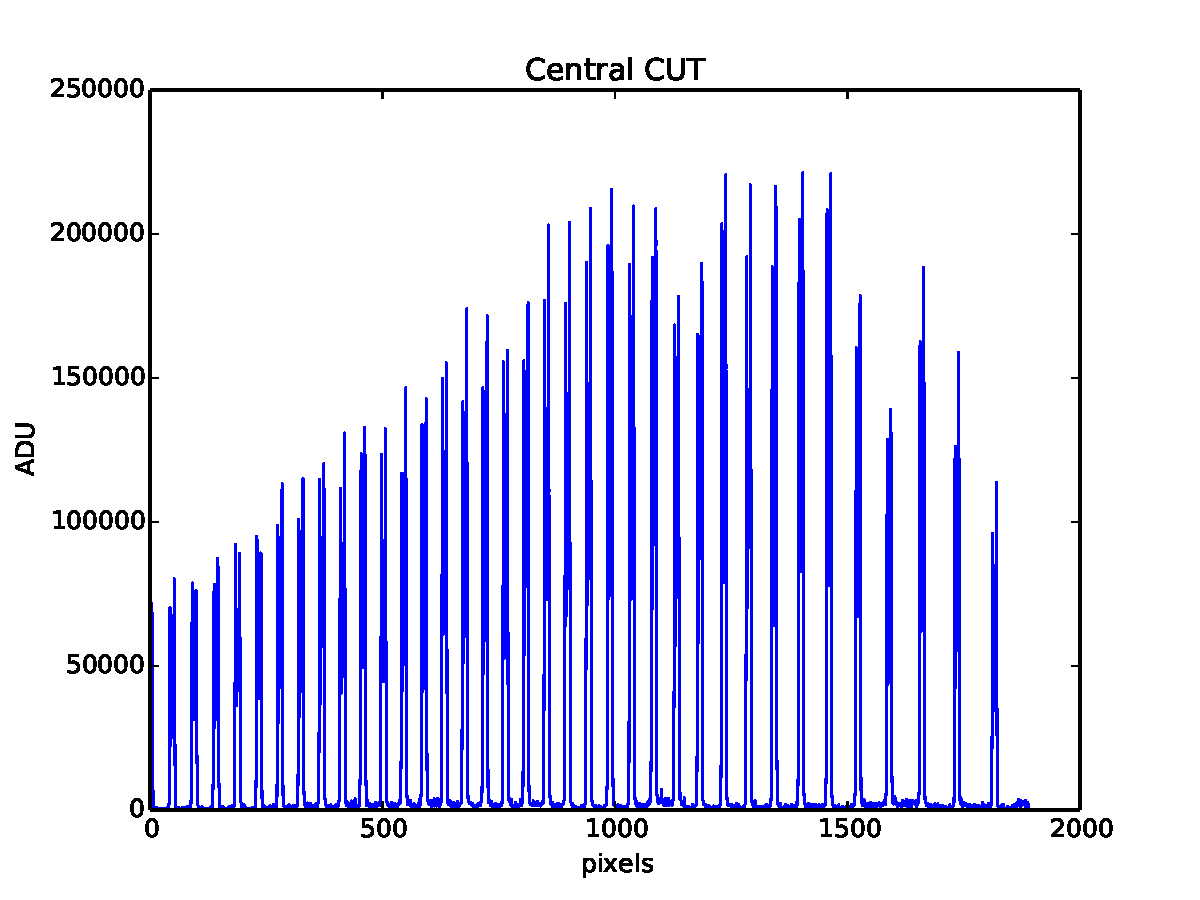
\includegraphics[width=.8\textwidth]{figures/cal_loc_RAW_spirou_1.pdf}
\caption{Pixel number (across order) against flux value of central pixel. \label{figure:cal_loc_RAW_spirou_1}}
\end{center}
\end{figure}

\begin{figure}
\begin{center}
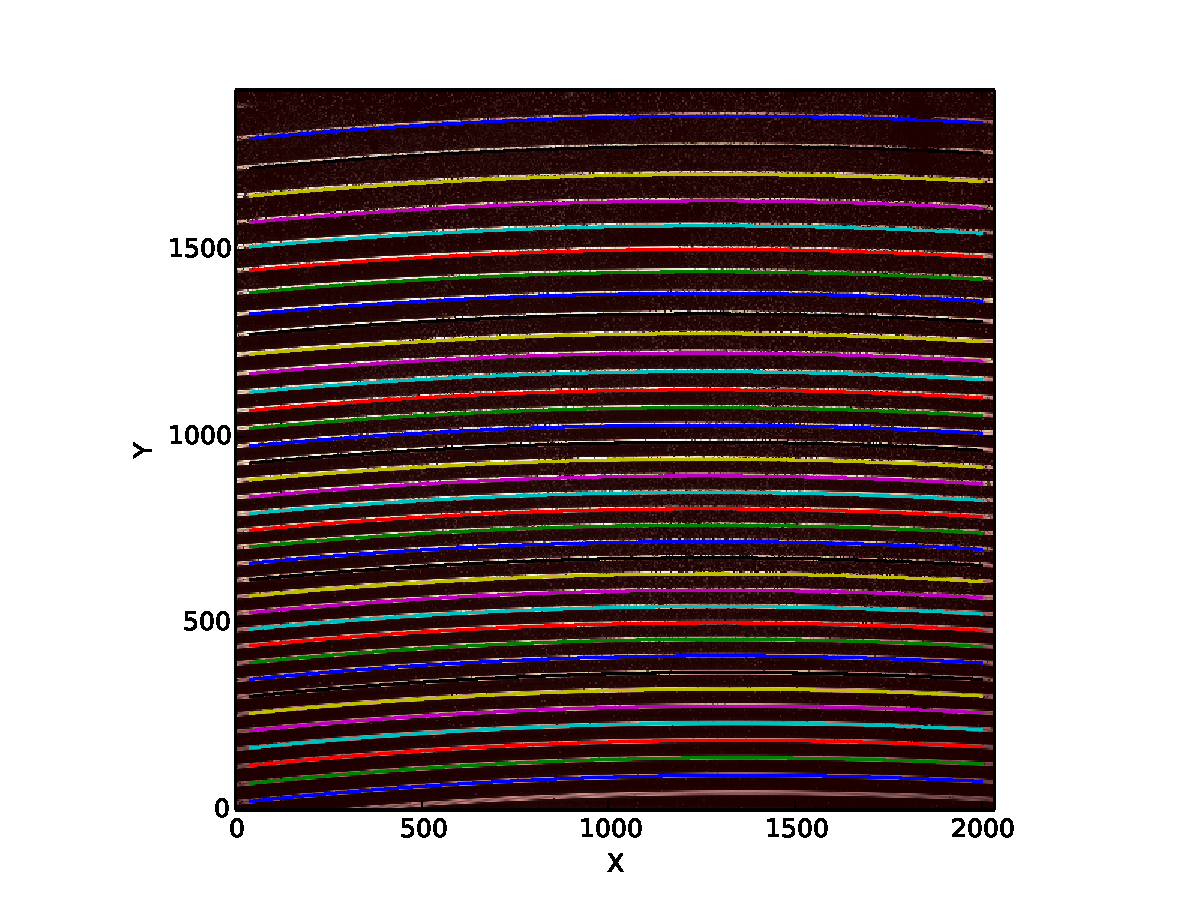
\includegraphics[width=.8\textwidth]{figures/cal_loc_RAW_spirou_2.pdf}
\caption{Image with fits to each order. \label{figure:cal_loc_RAW_spirou_2}}
\end{center}
\end{figure}

% ----------------------------------------------------------------------------------
\clearpage
\newpage
\section{The cal\_SLIT\_spirou recipe}
\label{section:cal_SLIT_spirou}
% ----------------------------------------------------------------------------------

Fabry-Perot exposures in which the three fibres are simultaneously fed by light from the Fabry-Perot filter. Each exposure is used to build the slit orientation. Finds the tilt of the orders. \\

% \TODO{Once writen up the new version update this description}

\noindent File prefixes allowed:
\begin{itemize}
	\item fp\_fp
\end{itemize}


\subsection{Summary of procedure}
\begin{enumerate}
\item adds all fp\_fp files together
\item corrects for dark
\item resizes the image
\item extracts the orders (no weight no tilt)
\item works out the tilt for each order using the location and width
\item saves the tilt to file
\item should do some quality control
\item  updates calibDB with key ``TILT''
\end{enumerate}

\subsection{Running cal\_}
To run cal\_ type:
\begin{lstlisting}[language=bash, style=bashstyle]
cal_SLIT_spirou.p  night_repository  filenames
\end{lstlisting}

\noindent Note: filesnames must start with `fp\_fp'

\subsection{Example working run}

An example run where everything worked is below:

\begin{lstlisting}[style=text]
cal_SLIT_spirou.py 20170710 fp_fp02a203.fits fp_fp03a203.fits fp_fp04a203.fits

||DRS  SPIROU   v   (interactive mode)
16:26:55.3 -   || *****************************************
16:26:55.3 -   || * SPIROU \@(#) Geneva Observatory ()
16:26:55.3 -   || *****************************************
16:26:55.3 -   ||(dir_data_raw)      DRS_DATA_RAW=/scratch/Projects/SPIRou_Pipeline/data/raw/
16:26:55.3 -   ||(dir_data_reduc)    DRS_DATA_REDUC=/scratch/Projects/SPIRou_Pipeline/data/reduced/
16:26:55.3 -   ||(dir_drs_config)    DRS_CONFIG=/scratch/Projects/SPIRou_Pipeline/INTROOT/DRS_SPIROU/config/
16:26:55.3 -   ||(dir_calib_db)      DRS_CALIB_DB=/scratch/Projects/SPIRou_Pipeline/data/calibDB
16:26:55.3 -   ||(dir_data_msg)      DRS_DATA_MSG=/scratch/Projects/SPIRou_Pipeline/data/msg/
16:26:55.3 -   ||(print_log)         DRS_LOG=1         %(0: minimum stdin-out logs)
16:26:55.3 -   ||(plot_graph)        DRS_PLOT=NONE            %(def/undef/trigger)
16:26:55.3 -   ||(used_date)         DRS_USED_DATE=undefined
16:26:55.3 -   ||(working_dir)       DRS_DATA_WORKING=/scratch/Projects/SPIRou_Pipeline/data/tmp/
16:26:55.3 -   ||                    DRS_INTERACTIVE is  set
16:26:55.3 -   |-c:+[...]|Now running : -c on file(s):  fp_fp02a203.fits fp_fp03a203.fits fp_fp04a203.fits
16:26:55.3 -   |-c:+[...]|On directory /scratch/Projects/SPIRou_Pipeline/data/raw/20170710
16:26:55.3 -   |-c:+[...]|ICDP loaded from: /scratch/Projects/SPIRou_Pipeline/INTROOT/DRS_SPIROU/config/hadmrICDP_SPIROU.py
16:26:55.4 -   |-c:+[...]|Calibration file: fp_fp02a203_tilt.fits already exists - not copied
16:26:55.4 -   |-c:+[...]|Calibration file: dark_flat02f10_loco_C.fits already exists - not copied
16:26:55.4 -   |-c:+[...]|Calibration file: dark_flat02f10_order_profil_C.fits already exists - not copied
16:26:55.5 -   |-c:+[...]|Calibration file: flat_dark02f10_order_profil_AB.fits already exists - not copied
16:26:55.5 -   |-c:+[...]|Calibration file: spirou_wave_ini3.fits already exists - not copied
16:26:55.5 -   |-c:+[...]|Calibration file: dark_dark02d406.fits already exists - not copied
16:26:55.5 -   |-c:+[...]|Calibration file: dark_flat02f10_flat_C.fits already exists - not copied
16:26:55.5 -   |-c:+[...]|Calibration file: flat_dark02f10_loco_AB.fits already exists - not copied
16:26:55.5 -   |-c:+[...]|Reading File: /scratch/Projects/SPIRou_Pipeline/data/raw/20170710/fp_fp02a203.fits
16:26:55.5 -   |-c:+[...]|Image 2048x2048 loaded
16:26:55.6 - * |-c:+[...]|Adding frames
16:26:55.6 -   |-c:+[...]|Reading File: /scratch/Projects/SPIRou_Pipeline/data/raw/20170710/fp_fp03a203.fits
16:26:55.6 -   |-c:+[...]|Reading File: /scratch/Projects/SPIRou_Pipeline/data/raw/20170710/fp_fp04a203.fits
16:26:55.9 -   |-c:+[...]|Doing Dark Correction using /scratch/Projects/SPIRou_Pipeline/data/calibDB/dark_dark02d406.fits
16:26:56.2 -   |-c:+[...]|Image format changed to 2035x1930
16:26:56.7 - * |-c:+[...]|Nb pixels morts = 611716 / 15.58 %
16:26:56.7 -   |-c:+[...]|Reading localization parameters of Fiber AB
16:26:57.0 -   |-c:+[...]|Order  0 : Tilt = 4.70 pixel sur 37.0 = -7.24 deg
16:26:57.2 -   |-c:+[...]|Order  1 : Tilt = 4.60 pixel sur 37.4 = -7.02 deg
16:26:57.4 -   |-c:+[...]|Order  2 : Tilt = 4.50 pixel sur 36.8 = -6.97 deg
16:26:57.6 -   |-c:+[...]|Order  3 : Tilt = 4.30 pixel sur 36.4 = -6.74 deg
16:26:57.8 -   |-c:+[...]|Order  4 : Tilt = 4.20 pixel sur 36.8 = -6.52 deg
16:26:58.0 -   |-c:+[...]|Order  5 : Tilt = 4.20 pixel sur 36.0 = -6.65 deg
16:26:58.2 -   |-c:+[...]|Order  6 : Tilt = 4.00 pixel sur 36.1 = -6.33 deg
16:26:58.4 -   |-c:+[...]|Order  7 : Tilt = 4.00 pixel sur 35.7 = -6.40 deg
16:26:58.6 -   |-c:+[...]|Order  8 : Tilt = 3.90 pixel sur 36.7 = -6.07 deg
16:26:58.8 -   |-c:+[...]|Order  9 : Tilt = 3.80 pixel sur 36.1 = -6.01 deg
16:26:59.0 -   |-c:+[...]|Order 10 : Tilt = 3.60 pixel sur 35.7 = -5.76 deg
16:26:59.3 -   |-c:+[...]|Order 11 : Tilt = 3.60 pixel sur 35.7 = -5.75 deg
16:26:59.5 -   |-c:+[...]|Order 12 : Tilt = 3.50 pixel sur 35.9 = -5.57 deg
16:26:59.7 -   |-c:+[...]|Order 13 : Tilt = 3.30 pixel sur 35.8 = -5.27 deg
16:26:59.8 -   |-c:+[...]|Order 14 : Tilt = 3.30 pixel sur 35.9 = -5.25 deg
16:27:00.0 -   |-c:+[...]|Order 15 : Tilt = 3.20 pixel sur 35.4 = -5.17 deg
16:27:00.2 -   |-c:+[...]|Order 16 : Tilt = 3.10 pixel sur 35.5 = -4.99 deg
16:27:00.3 -   |-c:+[...]|Order 17 : Tilt = 3.00 pixel sur 35.4 = -4.85 deg
16:27:00.5 -   |-c:+[...]|Order 18 : Tilt = 2.90 pixel sur 35.1 = -4.73 deg
16:27:00.7 -   |-c:+[...]|Order 19 : Tilt = 2.80 pixel sur 35.1 = -4.57 deg
16:27:00.8 -   |-c:+[...]|Order 20 : Tilt = 2.70 pixel sur 34.9 = -4.42 deg
16:27:01.0 -   |-c:+[...]|Order 21 : Tilt = 2.60 pixel sur 34.6 = -4.29 deg
16:27:01.2 -   |-c:+[...]|Order 22 : Tilt = 2.50 pixel sur 34.9 = -4.09 deg
16:27:01.3 -   |-c:+[...]|Order 23 : Tilt = 2.40 pixel sur 34.2 = -4.01 deg
16:27:01.5 -   |-c:+[...]|Order 24 : Tilt = 2.30 pixel sur 34.9 = -3.77 deg
16:27:01.7 -   |-c:+[...]|Order 25 : Tilt = 2.20 pixel sur 34.7 = -3.63 deg
16:27:01.8 -   |-c:+[...]|Order 26 : Tilt = 2.00 pixel sur 34.2 = -3.35 deg
16:27:02.0 -   |-c:+[...]|Order 27 : Tilt = 2.00 pixel sur 34.5 = -3.32 deg
16:27:02.2 -   |-c:+[...]|Order 28 : Tilt = 1.80 pixel sur 34.2 = -3.01 deg
16:27:02.3 -   |-c:+[...]|Order 29 : Tilt = 1.70 pixel sur 34.0 = -2.86 deg
16:27:02.5 -   |-c:+[...]|Order 30 : Tilt = 1.60 pixel sur 33.6 = -2.73 deg
16:27:02.7 -   |-c:+[...]|Order 31 : Tilt = 1.40 pixel sur 34.0 = -2.36 deg
16:27:02.8 -   |-c:+[...]|Order 32 : Tilt = 1.40 pixel sur 33.5 = -2.40 deg
16:27:03.0 -   |-c:+[...]|Order 33 : Tilt = 1.10 pixel sur 32.4 = -1.94 deg
16:27:03.2 -   |-c:+[...]|Order 34 : Tilt = 1.00 pixel sur 32.1 = -1.79 deg
16:27:03.3 -   |-c:+[...]|Order 35 : Tilt = 0.90 pixel sur 33.7 = -1.53 deg
16:27:03.3 - * |-c:+[...]AB|Tilt dispersion = 0.069 deg
16:27:03.6 -   |-c:+[...]|Saving tilt information in file: fp_fp02a203_tilt.fits
16:27:05.2 - * |-c:+[...]|Updating Calib Data Base with TILT
16:27:05.2 - * |-c:+[...]|Recipe -c has been successfully completed
\end{lstlisting}

\subsection{Interactive mode}

\begin{figure}
\begin{center}
\vcenteredhbox{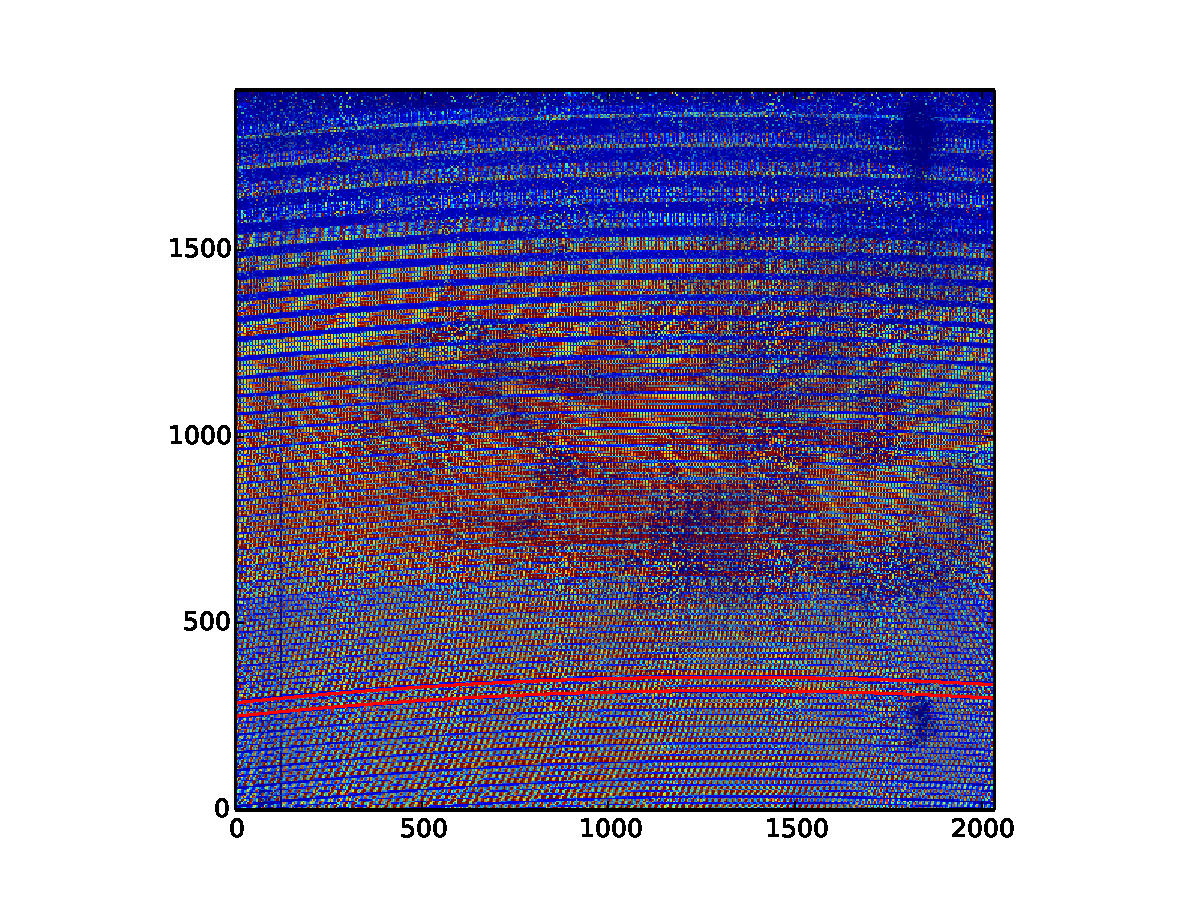
\includegraphics[width=.49\textwidth]{figures/cal_SLIT_spirou_1.pdf}}
\vcenteredhbox{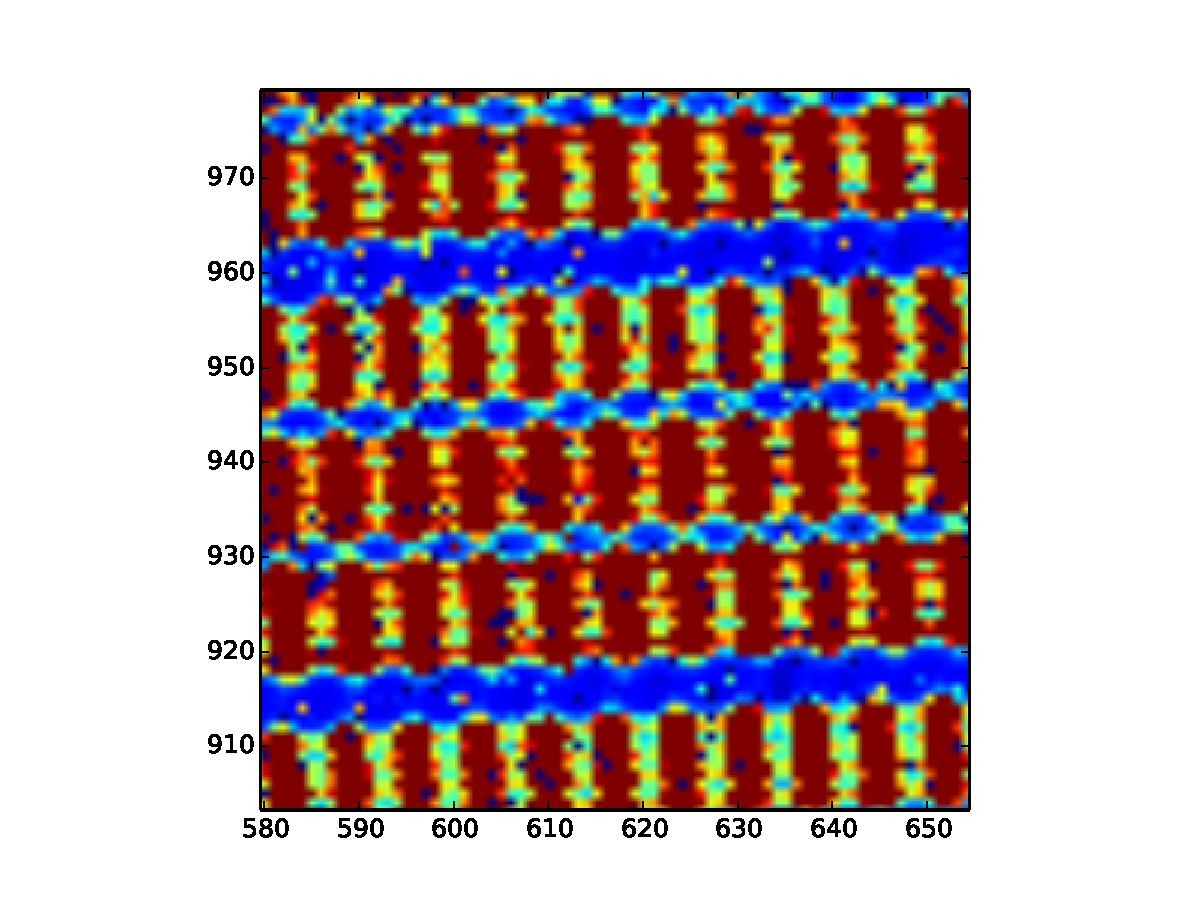
\includegraphics[width=.49\textwidth]{figures/cal_SLIT_spirou_1a.pdf}}
\caption{Left: The full `fp\_fp' image. Right: Zoom in on a section of the `fp\_fp' image showing the tilt.\label{figure:cal_slit_spirou_1}}
\end{center}
\end{figure}

\begin{figure}
\begin{center}
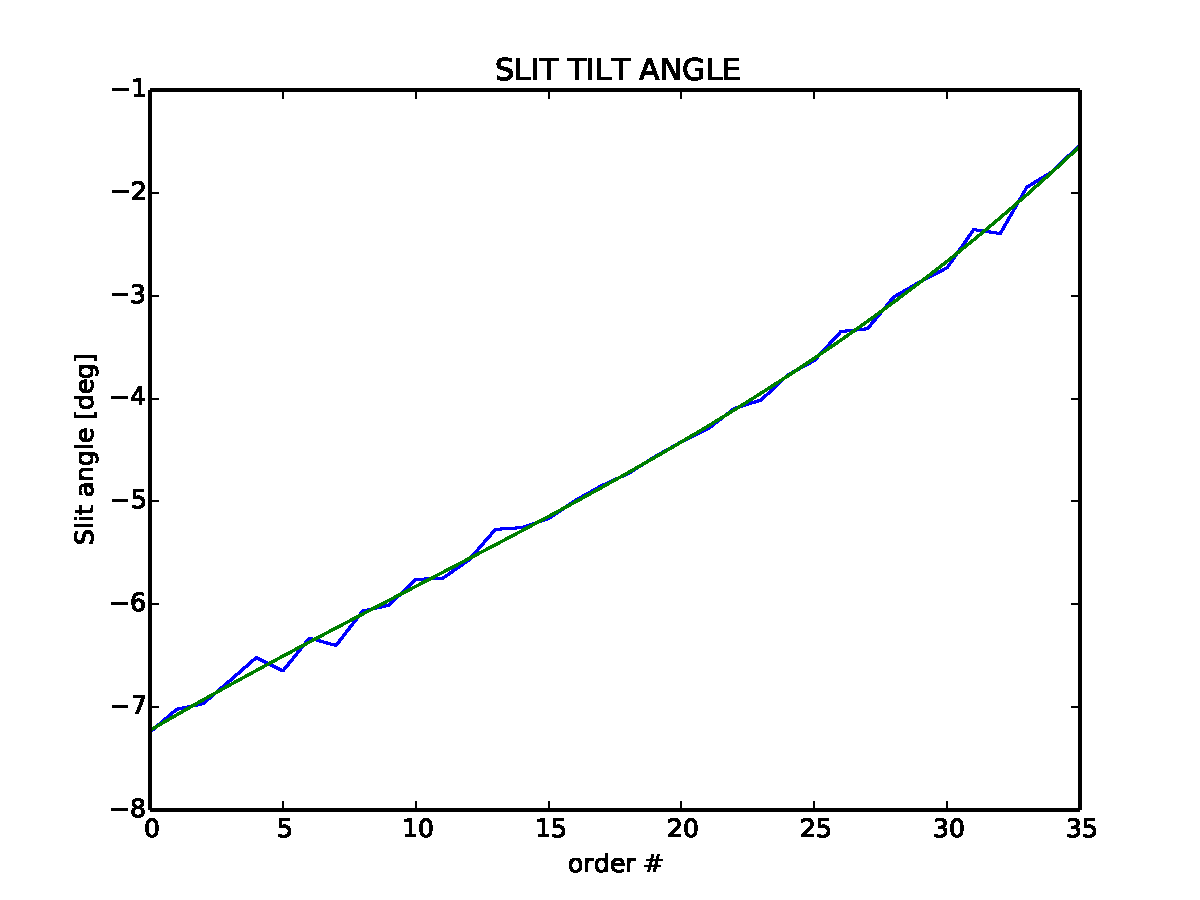
\includegraphics[width=.8\textwidth]{figures/cal_SLIT_spirou_2.pdf}
\caption{Slit aginle as a function of order number. \label{figure:cal_slit_spirou_2}}
\end{center}
\end{figure}

% ----------------------------------------------------------------------------------
\clearpage
\newpage
\section{The cal\_FF\_RAW\_spirou recipe}
\label{section:cal_FF_RAW_spirou}
% ----------------------------------------------------------------------------------

Creates the flat fields. \\ 

% \TODO{Once writen up the new version update this description} \\

\noindent File prefixes allowed:
\begin{itemize}
	\item dark\_flat
	\item flat\_dark
\end{itemize}

\noindent \textcolor{red}{Note: if using same files in Section \ref{section:working_example} you will get an error message when running the file}.
\noindent To solve this open the `master\_calib\_SPIROU.txt' file located in \textcolor{blue}{\{DATA\_ROOT\_CALIB\}}. Edit the unix date in the line that begins `TILT' so that it is less than the unix date on rwos `ORDER\_PROFIL\_AB' (i.e. change it from 1499707515.0 to 1499705515.0).

\noindent i.e. the `master\_calib\_SPIROU.txt' file should look go from
\begin{lstlisting}[style=text]
DARK 20170710 dark_dark02d406.fits 07/10/17/16:37:48 1499704668.0
ORDER_PROFIL_C 20170710 dark_flat02f10_order_profil_C.fits 07/10/17/17:03:50 1499706230.0
LOC_C 20170710 dark_flat02f10_loco_C.fits 07/10/17/17:03:50 1499706230.0
ORDER_PROFIL_AB 20170710 flat_dark02f10_order_profil_AB.fits 07/10/17/17:07:08 1499706428.0
LOC_AB 20170710 flat_dark02f10_loco_AB.fits 07/10/17/17:07:08 1499706428.0
TILT 20170710 fp_fp02a203_tilt.fits 07/10/17/17:25:15 @1499707515.0@
\end{lstlisting}

\noindent to this:

\definecolor{shadecolor}{named}{Tan} 
\begin{lstlisting}[style=text]
DARK 20170710 dark_dark02d406.fits 07/10/17/16:37:48 1499704668.0
ORDER_PROFIL_C 20170710 dark_flat02f10_order_profil_C.fits 07/10/17/17:03:50 1499706230.0
LOC_C 20170710 dark_flat02f10_loco_C.fits 07/10/17/17:03:50 1499706230.0
ORDER_PROFIL_AB 20170710 flat_dark02f10_order_profil_AB.fits 07/10/17/17:07:08 1499706428.0
LOC_AB 20170710 flat_dark02f10_loco_AB.fits 07/10/17/17:07:08 1499706428.0
TILT 20170710 fp_fp02a203_tilt.fits 07/10/17/17:25:15 @1499705515.0@

\end{lstlisting}

\subsection{Summary of procedure}
\begin{enumerate}
\item adds all `dark\_flat' or `flat\_dark' files together
\item corrects for darks
\item resizes the image
\item possible background subtraction?
\item extracts the orders using tilt and weight
\item calculates the blaze
\item calculates the flat field, (flat = extraction / blaze)
\item stores the flat fields
\item does some quality control
\item updates calibDB with key "FLAT\_\definekeyword{fiber}" where \definekeyword{fiber} = [AB, C] etc
\end{enumerate}

\subsection{Running cal\_FF\_RAW\_spirou}

To run cal\_FF\_RAW\_spirou type:
\begin{lstlisting}[language=bash, style=bashstyle]
cal_FF_RAW_spirou.py  night_repository  filenames
\end{lstlisting}

\noindent Note: filenames must start with `dark\_flat' or `flat\_dark'

\subsection{Example working run}

An example run where everything worked is below:

\begin{lstlisting}[style=text]
cal_FF_RAW_spirou.py 20170710 dark_flat02f10.fits dark_flat03f10.fits
dark_flat04f10.fits dark_flat05f10.fits dark_flat06f10.fits

||DRS  SPIROU   v   (interactive mode)
16:49:40.5 -   || *****************************************
16:49:40.5 -   || * SPIROU \@(#) Geneva Observatory ()
16:49:40.5 -   || *****************************************
16:49:40.5 -   ||(dir_data_raw)      DRS_DATA_RAW=/scratch/Projects/SPIRou_Pipeline/data/raw/
16:49:40.5 -   ||(dir_data_reduc)    DRS_DATA_REDUC=/scratch/Projects/SPIRou_Pipeline/data/reduced/
16:49:40.5 -   ||(dir_drs_config)    DRS_CONFIG=/scratch/Projects/SPIRou_Pipeline/INTROOT/DRS_SPIROU/config/
16:49:40.5 -   ||(dir_calib_db)      DRS_CALIB_DB=/scratch/Projects/SPIRou_Pipeline/data/calibDB
16:49:40.5 -   ||(dir_data_msg)      DRS_DATA_MSG=/scratch/Projects/SPIRou_Pipeline/data/msg/
16:49:40.5 -   ||(print_log)         DRS_LOG=1         %(0: minimum stdin-out logs)
16:49:40.5 -   ||(plot_graph)        DRS_PLOT=NONE            %(def/undef/trigger)
16:49:40.5 -   ||(used_date)         DRS_USED_DATE=undefined
16:49:40.5 -   ||(working_dir)       DRS_DATA_WORKING=/scratch/Projects/SPIRou_Pipeline/data/tmp/
16:49:40.5 -   ||                    DRS_INTERACTIVE is  set
16:49:40.5 -   |-c:+[...]|Now running : -c on file(s):  dark_flat02f10.fits dark_flat03f10.fits
16:49:40.5 -   |-c:+[...]|On directory /scratch/Projects/SPIRou_Pipeline/data/raw/20170710
16:49:40.5 -   |-c:+[...]|ICDP loaded from: /scratch/Projects/SPIRou_Pipeline/INTROOT/DRS_SPIROU/config/hadmrICDP_SPIROU.py
16:49:40.5 - * |-c:+[...]|Now processing Image TYPE: UNKNOWN  with -c recipe
16:49:40.6 -   |-c:+[...]|Calibration file: dark_dark02d406.fits already exists - not copied
16:49:40.6 -   |-c:+[...]|Calibration file: fp_fp02a203_tilt.fits already exists - not copied
16:49:40.6 -   |-c:+[...]|Reading File: /scratch/Projects/SPIRou_Pipeline/data/raw/20170710/dark_flat02f10.fits
16:49:40.6 -   |-c:+[...]|Image 2048x2048 loaded
16:49:40.6 - * |-c:+[...]|Adding frames
16:49:40.6 -   |-c:+[...]|Reading File: /scratch/Projects/SPIRou_Pipeline/data/raw/20170710/dark_flat03f10.fits
16:49:40.7 -   |-c:+[...]|Doing Dark Correction using /scratch/Projects/SPIRou_Pipeline/data/calibDB/dark_dark02d406.fits
16:49:41.0 -   |-c:+[...]|Image format changed to 2035x1930
16:49:41.5 - * |-c:+[...]|Nb pixels morts = 568533 / 14.48 %
16:49:41.5 - * |-c:+[...]|Maximum average flux/pixel in the spectrum: 73264.1[ADU]
16:49:41.5 -   |-c:+[...]|Reading tilt slit 
16:49:41.5 -   |-c:+[...]C|Reading localization parameters of Fiber C
16:49:41.6 -   |-c:+[...]C|Reading order profil of Fiber C
16:49:42.1 -   |-c:+[...]|On fiber C  order  0: S/N= 685.6  - FF rms= 4.68 %
16:49:42.7 -   |-c:+[...]|On fiber C  order  1: S/N= 709.3  - FF rms= 4.81 %
16:49:43.3 -   |-c:+[...]|On fiber C  order  2: S/N= 733.7  - FF rms= 4.75 %
16:49:43.8 -   |-c:+[...]|On fiber C  order  3: S/N= 759.2  - FF rms= 4.86 %
16:49:44.4 -   |-c:+[...]|On fiber C  order  4: S/N= 780.7  - FF rms= 4.94 %
16:49:44.9 -   |-c:+[...]|On fiber C  order  5: S/N= 811.4  - FF rms= 5.03 %
16:49:45.5 -   |-c:+[...]|On fiber C  order  6: S/N= 842.1  - FF rms= 5.11 %
16:49:46.0 -   |-c:+[...]|On fiber C  order  7: S/N= 875.4  - FF rms= 5.23 %
16:49:46.6 -   |-c:+[...]|On fiber C  order  8: S/N= 893.9  - FF rms= 5.37 %
16:49:47.2 -   |-c:+[...]|On fiber C  order  9: S/N= 916.4  - FF rms= 6.07 %
16:49:47.7 -   |-c:+[...]|On fiber C  order 10: S/N= 928.3  - FF rms= 8.02 %
16:49:48.3 -   |-c:+[...]|On fiber C  order 11: S/N= 912.5  - FF rms= 6.84 %
16:49:48.8 -   |-c:+[...]|On fiber C  order 12: S/N= 961.8  - FF rms= 5.94 %
16:49:49.4 -   |-c:+[...]|On fiber C  order 13: S/N= 1004.9  - FF rms= 5.97 %
16:49:49.9 -   |-c:+[...]|On fiber C  order 14: S/N= 1022.5  - FF rms= 6.15 %
16:49:50.5 -   |-c:+[...]|On fiber C  order 15: S/N= 1045.5  - FF rms= 6.18 %
16:49:51.1 -   |-c:+[...]|On fiber C  order 16: S/N= 1053.4  - FF rms= 6.14 %
16:49:51.6 -   |-c:+[...]|On fiber C  order 17: S/N= 1085.8  - FF rms= 6.23 %
16:49:52.2 -   |-c:+[...]|On fiber C  order 18: S/N= 1103.0  - FF rms= 6.28 %
16:49:52.7 -   |-c:+[...]|On fiber C  order 19: S/N= 1134.8  - FF rms= 6.77 %
16:49:53.3 -   |-c:+[...]|On fiber C  order 20: S/N= 1150.4  - FF rms= 6.43 %
16:49:53.9 -   |-c:+[...]|On fiber C  order 21: S/N= 1144.2  - FF rms= 6.42 %
16:49:54.4 -   |-c:+[...]|On fiber C  order 22: S/N= 1139.6  - FF rms= 6.39 %
16:49:55.0 -   |-c:+[...]|On fiber C  order 23: S/N= 1161.3  - FF rms= 6.52 %
16:49:55.5 -   |-c:+[...]|On fiber C  order 24: S/N= 1137.8  - FF rms= 9.11 %
16:49:56.1 -   |-c:+[...]|On fiber C  order 25: S/N= 1131.4  - FF rms= 9.39 %
16:49:56.6 -   |-c:+[...]|On fiber C  order 26: S/N= 1113.7  - FF rms= 7.97 %
16:49:57.2 -   |-c:+[...]|On fiber C  order 27: S/N= 1161.7  - FF rms= 6.04 %
16:49:57.7 -   |-c:+[...]|On fiber C  order 28: S/N= 1153.9  - FF rms= 6.07 %
16:49:58.3 -   |-c:+[...]|On fiber C  order 29: S/N= 1178.2  - FF rms= 5.89 %
16:49:58.9 -   |-c:+[...]|On fiber C  order 30: S/N= 1150.4  - FF rms= 5.92 %
16:49:59.6 -   |-c:+[...]|On fiber C  order 31: S/N= 1024.1  - FF rms= 5.60 %
16:50:00.3 -   |-c:+[...]|On fiber C  order 32: S/N= 945.1  - FF rms= 5.60 %
16:50:01.0 -   |-c:+[...]|On fiber C  order 33: S/N= 1030.4  - FF rms= 5.70 %
16:50:01.6 -   |-c:+[...]|On fiber C  order 34: S/N= 957.7  - FF rms= 8.21 %
16:50:02.2 -   |-c:+[...]|On fiber C  order 35: S/N= 753.1  - FF rms= 8.11 %
16:50:02.4 -   |-c:+[...]C|Saving blaze spectrum for fiber: C in dark_flat02f10_blaze_C.fits
16:50:03.1 -   |-c:+[...]C|Saving FF  spectrum of Fiber C in dark_flat02f10_flat_C.fits
16:50:04.2 - * |-c:+[...]|Updating Calib Data Base with FLAT_C
16:50:04.2 - * |-c:+[...]|Recipe -c has been  successfully completed
\end{lstlisting}

\subsection{Interactive mode}

\begin{figure}
\begin{center}
\vcenteredhbox{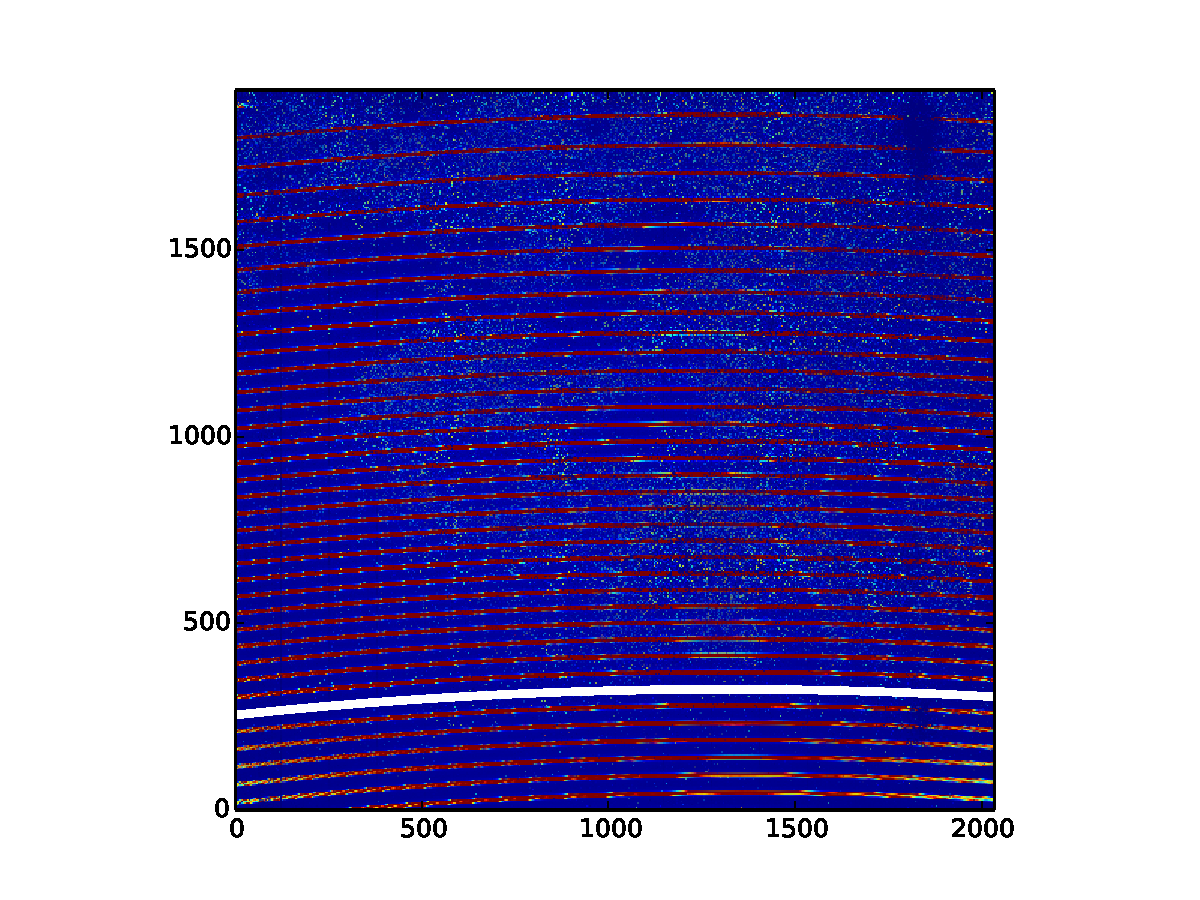
\includegraphics[width=.49\textwidth]{figures/cal_FF_RAW_spirou_1.pdf}}
\vcenteredhbox{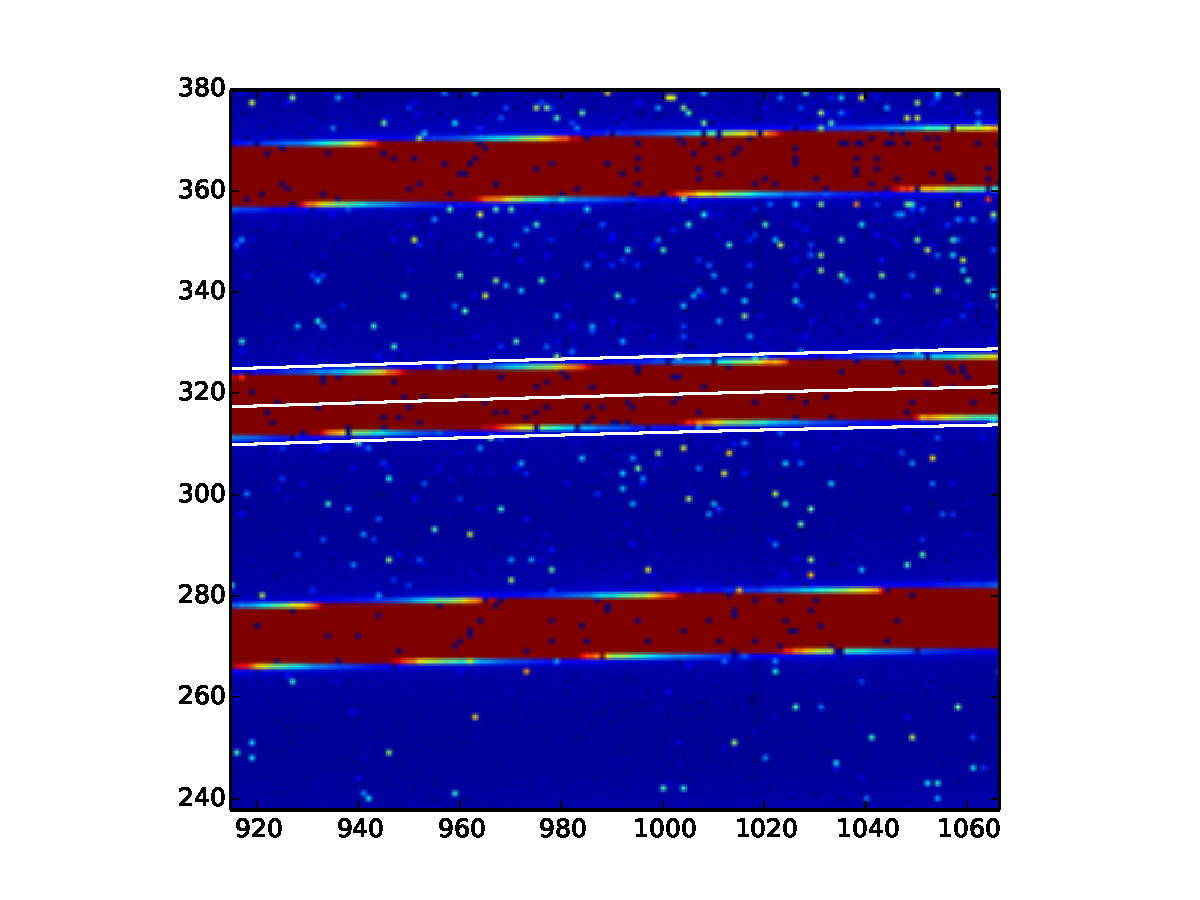
\includegraphics[width=.49\textwidth]{figures/cal_FF_RAW_spirou_1a.pdf}}
\caption{Left: the full processed image with one order fit highlighted. Right: Zoom in of the highlighted order fit. \label{figure:cal_FF_RAW_spirou_1}}
\end{center}
\end{figure}

\begin{figure}
\begin{center}
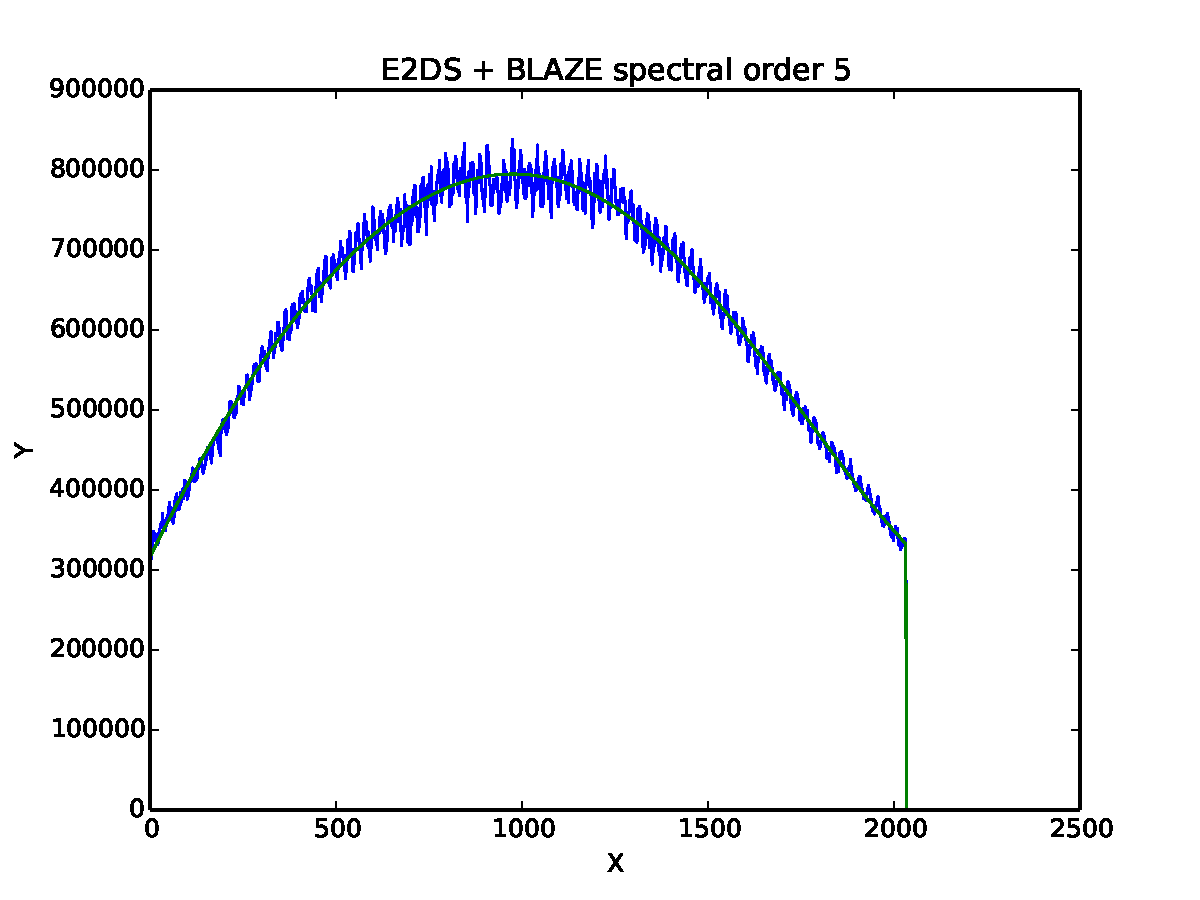
\includegraphics[width=.8\textwidth]{figures/cal_FF_RAW_spirou_2.pdf}
\caption{The extracted highlighted order from Figure \protect\ref{figure:cal_FF_RAW_spirou_1}. Overplotted is the blaze fit (in cyan). \label{figure:cal_FF_RAW_spirou_2}}
\end{center}
\end{figure}

\begin{figure}
\begin{center}
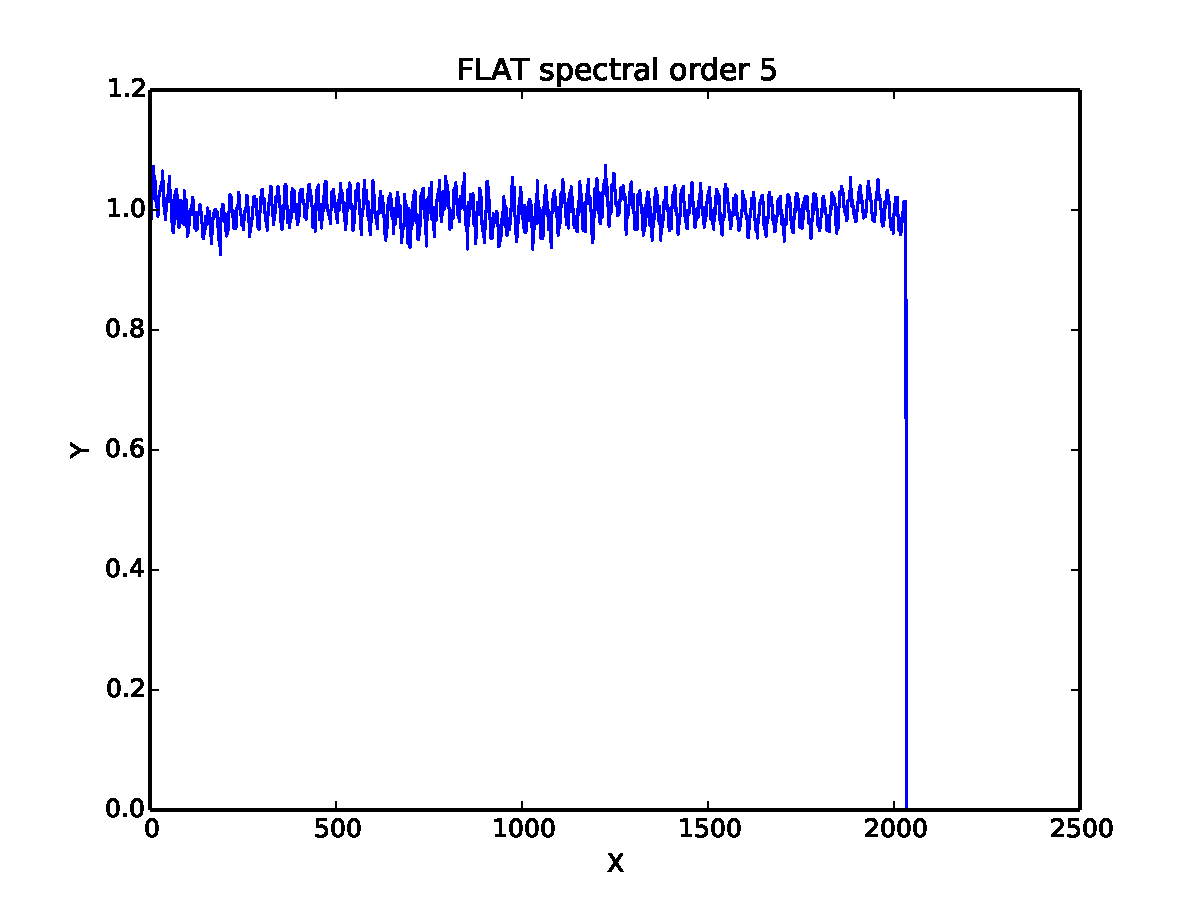
\includegraphics[width=.8\textwidth]{figures/cal_FF_RAW_spirou_3.pdf}
\caption{The flattened order for highlighted order from Figure \protect\ref{figure:cal_FF_RAW_spirou_1}. \label{figure:cal_FF_RAW_spirou_3}}
\end{center}
\end{figure}

% ----------------------------------------------------------------------------------
\clearpage
\newpage
\section{The cal\_extract\_RAW\_spirou recipe}
\label{section:cal_extract_RAW_spirou}
% ----------------------------------------------------------------------------------

Extracts orders for specific fibers and files. \\

\noindent File prefixes allowed:
\begin{itemize}
	\item fp\_fp
	\item hcone\_dark
	\item dark\_hcone
	\item hcone\_hcone
	\item dark\_dark\_AHC1
	\item dark\_hctwo
	\item hctwo\_hctwo
	\item dark\_dark\_AHC2
\end{itemize}

% \TODO{Once writen up the new version update this description}

\subsection{Summary of procedure}
\begin{enumerate}
\item adds all files together
\item corrects for darks
\item resizes the image
\item checks for saturation
\item possible background subtraction?
\item extracts orders
	\begin{itemize}
		\item without tilt/weight fortran
		\item without tilt/weight python
		\item with tilt (no weight)
		\item with tilt and weight
		\item with weight (no tilt)
	\end{itemize}
\item saves extraction with weight (no tilt) to e2ds file
\end{enumerate}

\subsection{Running cal\_extract\_RAW\_spirou}

To run cal\_extract\_RAW\_spirou on fiber=AB:
\begin{lstlisting}[language=bash, style=bashstyle]
cal_extract_RAW_spirouAB.py  night_repository  filenames
\end{lstlisting}
To run cal\_extract\_RAW\_spirou on fiber=C:
\begin{lstlisting}[language=bash, style=bashstyle]
cal_extract_RAW_spirouC.py  night_repository  filenames
\end{lstlisting}

Note: Filenames must start with `fp\_fp', `hcone\_dark', `dark\_hcone', `hcone\_hcone', `dark\_dark\_AHC1', `dark\_hctwo', `hctwo\_hctwo', or `dark\_dark\_AHC2'.


\subsection{Example working run}

An example run where everything worked is below:

\begin{lstlisting}[style=text]
cal_extract_RAW_spirouC.py 20170710 fp_fp02a203.fits fp_fp03a203.fits
fp_fp04a203.fits

||DRS  SPIROU   v   (interactive mode)
17:38:04.5 -   || *****************************************
17:38:04.5 -   || * SPIROU \@(#) Geneva Observatory ()
17:38:04.5 -   || *****************************************
17:38:04.5 -   ||(dir_data_raw)      DRS_DATA_RAW=/scratch/Projects/SPIRou_Pipeline/data/raw/
17:38:04.5 -   ||(dir_data_reduc)    DRS_DATA_REDUC=/scratch/Projects/SPIRou_Pipeline/data/reduced/
17:38:04.5 -   ||(dir_drs_config)    DRS_CONFIG=/scratch/Projects/SPIRou_Pipeline/INTROOT/DRS_SPIROU/config/
17:38:04.5 -   ||(dir_calib_db)      DRS_CALIB_DB=/scratch/Projects/SPIRou_Pipeline/data/calibDB
17:38:04.5 -   ||(dir_data_msg)      DRS_DATA_MSG=/scratch/Projects/SPIRou_Pipeline/data/msg/
17:38:04.5 -   ||(print_log)         DRS_LOG=1         %(0: minimum stdin-out logs)
17:38:04.5 -   ||(plot_graph)        DRS_PLOT=NONE            %(def/undef/trigger)
17:38:04.5 -   ||(used_date)         DRS_USED_DATE=undefined
17:38:04.5 -   ||(working_dir)       DRS_DATA_WORKING=/scratch/Projects/SPIRou_Pipeline/data/tmp/
17:38:04.5 -   ||                    DRS_INTERACTIVE is  set
17:38:04.5 -   |-c:+[...]|Now running : -c on file(s):  fp_fp02a203.fits fp_fp03a203.fits
17:38:04.5 -   |-c:+[...]|On directory /scratch/Projects/SPIRou_Pipeline/data/raw/20170710
17:38:04.5 -   |-c:+[...]|ICDP loaded from: /scratch/Projects/SPIRou_Pipeline/INTROOT/DRS_SPIROU/config/hadmrICDP_SPIROU.py
17:38:04.5 - * |-c:+[...]|Now processing Image TYPE: UNKNOWN  with -c recipe
17:38:04.6 -   |-c:+[...]|Calibration file: fp_fp02a203_tilt.fits already exists - not copied
17:38:04.6 -   |-c:+[...]|Calibration file: dark_flat02f10_loco_C.fits already exists - not copied
17:38:04.6 -   |-c:+[...]|Calibration file: flat_dark02f10_order_profil_AB.fits already exists - not copied
17:38:04.6 -   |-c:+[...]|Calibration file: spirou_wave_ini3.fits already exists - not copied
17:38:04.7 -   |-c:+[...]|Calibration file: dark_dark02d406.fits already exists - not copied
17:38:04.7 -   |-c:+[...]|Calibration file: dark_flat02f10_flat_C.fits already exists - not copied
17:38:04.7 -   |-c:+[...]|Calibration file: dark_flat02f10_order_profil_C.fits already exists - not copied
17:38:04.7 -   |-c:+[...]|Calibration file: flat_dark02f10_loco_AB.fits already exists - not copied
17:38:04.7 -   |-c:+[...]|Reading File: /scratch/Projects/SPIRou_Pipeline/data/raw/20170710/fp_fp02a203.fits
17:38:04.7 -   |-c:+[...]|Image 2048x2048 loaded
17:38:04.8 - * |-c:+[...]|Adding frames
17:38:04.8 -   |-c:+[...]|Reading File: /scratch/Projects/SPIRou_Pipeline/data/raw/20170710/fp_fp03a203.fits
17:38:04.9 -   |-c:+[...]|Doing Dark Correction using /scratch/Projects/SPIRou_Pipeline/data/calibDB/dark_dark02d406.fits
17:38:05.1 -   |-c:+[...]|Image format changed to 2035x1930
17:38:05.6 - * |-c:+[...]|Nb pixels morts = 568485 / 14.47 %
17:38:05.6 - * |-c:+[...]|Maximum average flux/pixel in the spectrum: 110446.0[ADU]
17:38:05.6 -   |-c:+[...]|Reading tilt slit 
17:38:05.7 -   |-c:+[...]|Reading wavelength solution 
17:38:05.7 -   |-c:+[...]C|Reading localization parameters of Fiber C
17:38:05.7 -   |-c:+[...]C|Reading order profil of Fiber C
17:38:07.1 -   |-c:+[...]|On fiber C  order  0: S/N= 712.0  
17:38:08.9 -   |-c:+[...]|On fiber C  order  1: S/N= 780.2  
17:38:10.3 -   |-c:+[...]|On fiber C  order  2: S/N= 726.0  
17:38:12.0 -   |-c:+[...]|On fiber C  order  3: S/N= 700.3  
17:38:13.5 -   |-c:+[...]|On fiber C  order  4: S/N= 702.3  
17:38:14.9 -   |-c:+[...]|On fiber C  order  5: S/N= 740.0  
17:38:16.3 -   |-c:+[...]|On fiber C  order  6: S/N= 773.4  
17:38:17.7 -   |-c:+[...]|On fiber C  order  7: S/N= 758.5  
17:38:19.2 -   |-c:+[...]|On fiber C  order  8: S/N= 752.0  
17:38:20.7 -   |-c:+[...]|On fiber C  order  9: S/N= 763.0  
17:38:22.1 -   |-c:+[...]|On fiber C  order 10: S/N= 794.5  
17:38:23.5 -   |-c:+[...]|On fiber C  order 11: S/N= 671.5  
17:38:25.2 -   |-c:+[...]|On fiber C  order 12: S/N= 871.4  
17:38:26.7 -   |-c:+[...]|On fiber C  order 13: S/N= 883.0  
17:38:28.4 -   |-c:+[...]|On fiber C  order 14: S/N= 1070.7  
17:38:29.9 -   |-c:+[...]|On fiber C  order 15: S/N= 954.4  
17:38:31.6 -   |-c:+[...]|On fiber C  order 16: S/N= 909.4
17:38:33.3 -   |-c:+[...]|On fiber C  order 17: S/N= 935.8
17:38:34.9 -   |-c:+[...]|On fiber C  order 18: S/N= 905.3
17:38:36.4 -   |-c:+[...]|On fiber C  order 19: S/N= 888.5
17:38:37.8 -   |-c:+[...]|On fiber C  order 20: S/N= 896.3
17:38:39.6 -   |-c:+[...]|On fiber C  order 21: S/N= 888.1
17:38:41.3 -   |-c:+[...]|On fiber C  order 22: S/N= 848.4
17:38:43.0 -   |-c:+[...]|On fiber C  order 23: S/N= 860.3
17:38:44.7 -   |-c:+[...]|On fiber C  order 24: S/N= 817.9
17:38:46.1 -   |-c:+[...]|On fiber C  order 25: S/N= 813.0
17:38:47.5 -   |-c:+[...]|On fiber C  order 26: S/N= 792.2
17:38:49.0 -   |-c:+[...]|On fiber C  order 27: S/N= 836.9
17:38:50.7 -   |-c:+[...]|On fiber C  order 28: S/N= 882.4
17:38:52.3 -   |-c:+[...]|On fiber C  order 29: S/N= 837.6
17:38:53.7 -   |-c:+[...]|On fiber C  order 30: S/N= 785.7
17:38:55.1 -   |-c:+[...]|On fiber C  order 31: S/N= 434.9
17:38:56.5 -   |-c:+[...]|On fiber C  order 32: S/N= 376.3
17:38:58.0 -   |-c:+[...]|On fiber C  order 33: S/N= 614.3
17:38:59.7 -   |-c:+[...]|On fiber C  order 34: S/N= 523.1
17:39:01.2 -   |-c:+[...]|On fiber C  order 35: S/N= 343.2
17:39:01.5 -   |-c:+[...]|Saving E2DS spectrum of Fiber C in fp_fp02a203_e2ds_C.fits
17:39:02.1 - * |-c:+[...]|Recipe -c has been  successfully completed
\end{lstlisting}

\subsection{Interactive mode}

\begin{figure}
\begin{center}
\vcenteredhbox{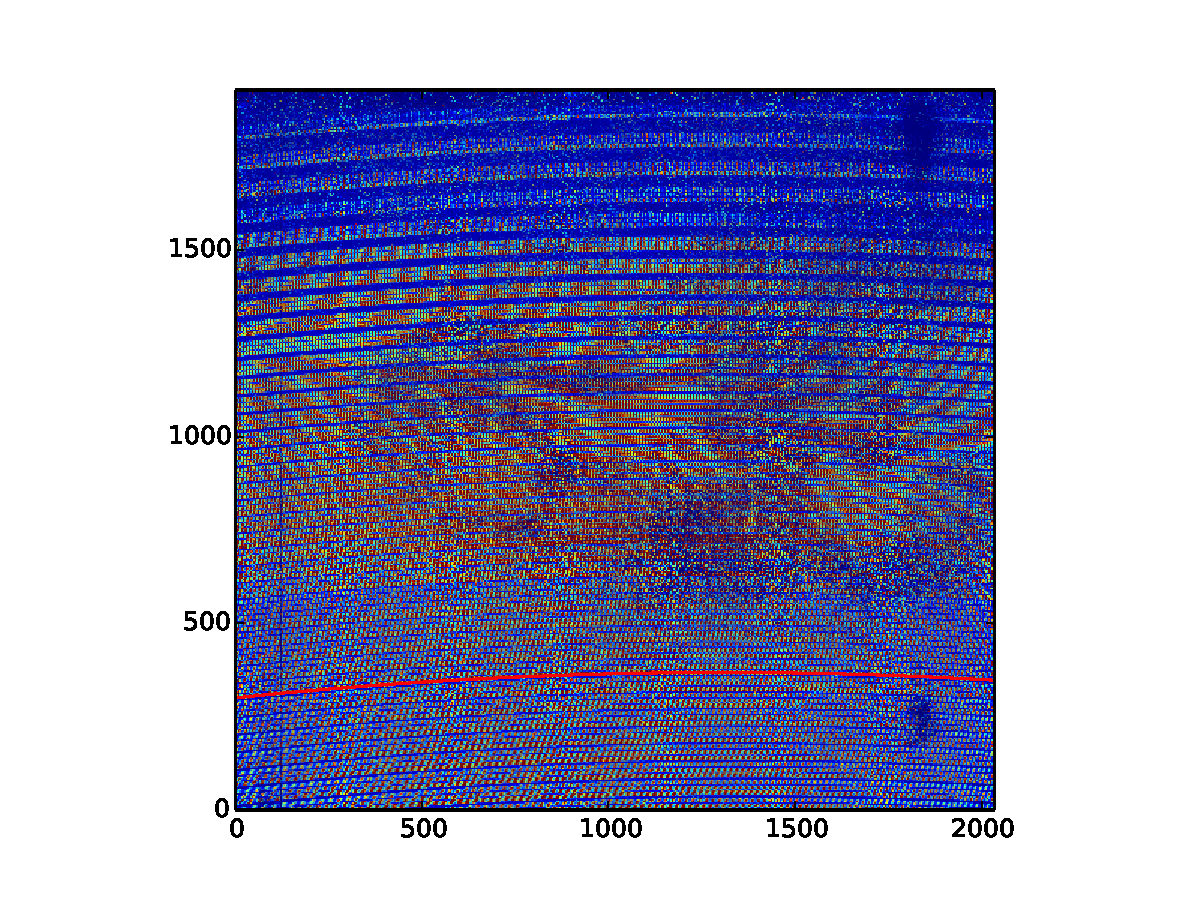
\includegraphics[width=.49\textwidth]{figures/cal_extract_RAW_spirou_1.pdf}}
\vcenteredhbox{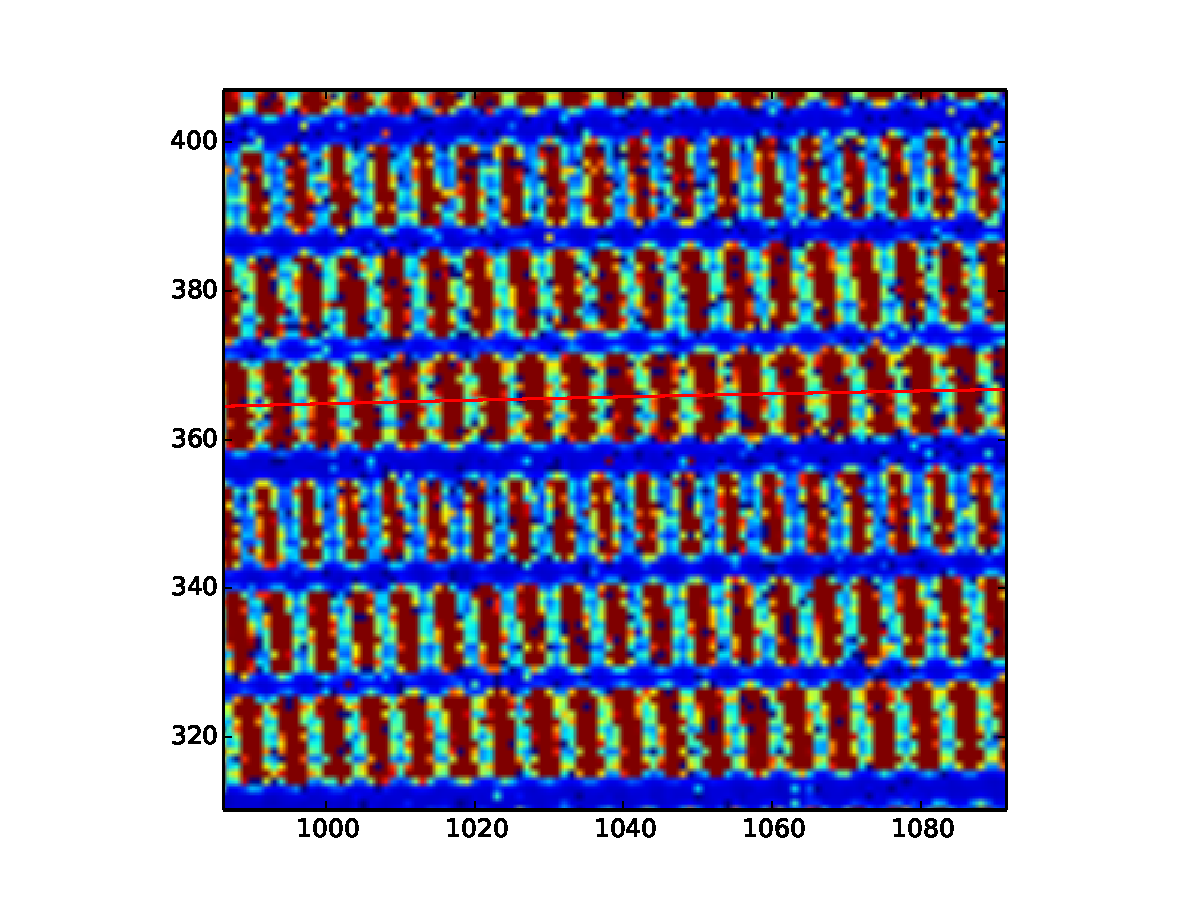
\includegraphics[width=.49\textwidth]{figures/cal_extract_RAW_spirou_1a.pdf}}
\caption{Left: The full process image. Right: Zoom in on the highlighted spectral order fit. \label{figure:cal_extract_RAW_spirou_1}}
\end{center}
\end{figure}

\begin{figure}
\begin{center}
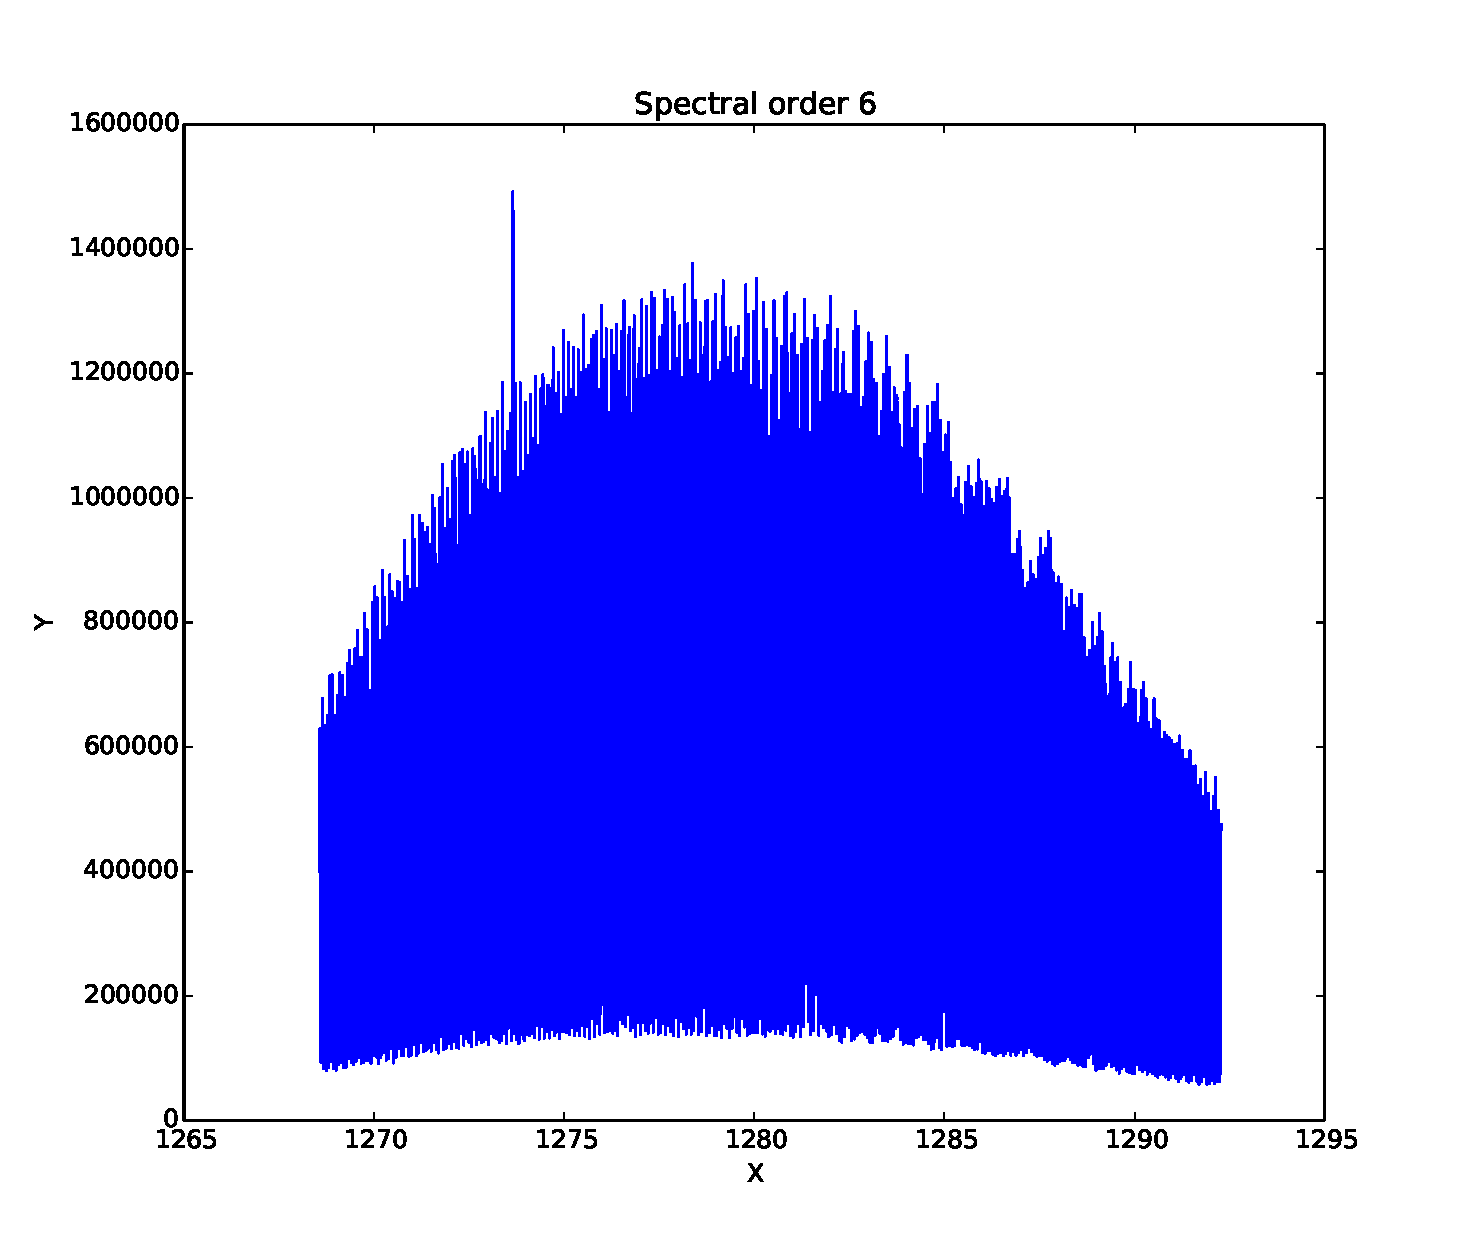
\includegraphics[width=.8\textwidth]{figures/cal_extract_RAW_spirou_2.pdf}
\caption{The extract spectrum from the hightlighted spectral order in \protect\ref{figure:cal_extract_RAW_spirou_1}. \label{figure:cal_extract_RAW_spirou_2}}
\end{center}
\end{figure}

% ----------------------------------------------------------------------------------
\clearpage
\newpage
\section{The cal\_DRIFT\_RAW\_spirou recipe}
\label{section:cal_DRIFT_RAW_spirou}
% ----------------------------------------------------------------------------------

Calculates relative (radial velocity) drift between all files and individual files. \\

% \TODO{Once writen up the new version update this description}

\noindent File prefixes allowed:
\begin{itemize}
	\item fp\_fp
\end{itemize}

\subsection{Summary of procedure}
\begin{enumerate}
	\item first file is reference image
	\item resizes the image
	\item extracts with weight (no tilt)
	\item loops around all other `fp\_fp' files in directory
	\item calculates photon noise uncertainty and estimated RV uncertainty on spectrum
	\begin{itemize}
		\item uses wave file
	\end{itemize}
	\item calculates RV drift and mean RV drift between reference (mean of files) and other `fp\_fp' files
	\item saves drift values to file
\end{enumerate}

\subsection{Running cal\_DRIFT\_RAW\_spirou}

To run cal\_DRIFT\_RAW\_spirou type:
\begin{lstlisting}[language=bash, style=bashstyle]
cal_DRIFT_RAW_spirou.py  night_repository  filenames
\end{lstlisting}

Note: Filenames must start with `fp\_fp'.

\subsection{Example working run}

An example run where everything worked is below:

\begin{lstlisting}[style=text]
cal_DRIFT_RAW_spirou.py 20170710 fp_fp02a203.fits fp_fp03a203.fits
fp_fp04a203.fits

||DRS  SPIROU   v   (interactive mode)
17:58:26.1 -   || *****************************************
17:58:26.1 -   || * SPIROU \@(#) Geneva Observatory ()
17:58:26.1 -   || *****************************************
17:58:26.1 -   ||(dir_data_raw)      DRS_DATA_RAW=/scratch/Projects/SPIRou_Pipeline/data/raw/
17:58:26.1 -   ||(dir_data_reduc)    DRS_DATA_REDUC=/scratch/Projects/SPIRou_Pipeline/data/reduced/
17:58:26.1 -   ||(dir_drs_config)    DRS_CONFIG=/scratch/Projects/SPIRou_Pipeline/INTROOT/DRS_SPIROU/config/
17:58:26.1 -   ||(dir_calib_db)      DRS_CALIB_DB=/scratch/Projects/SPIRou_Pipeline/data/calibDB
17:58:26.1 -   ||(dir_data_msg)      DRS_DATA_MSG=/scratch/Projects/SPIRou_Pipeline/data/msg/
17:58:26.1 -   ||(print_log)         DRS_LOG=1         %(0: minimum stdin-out logs)
17:58:26.1 -   ||(plot_graph)        DRS_PLOT=NONE            %(def/undef/trigger)
17:58:26.1 -   ||(used_date)         DRS_USED_DATE=undefined
17:58:26.1 -   ||(working_dir)       DRS_DATA_WORKING=/scratch/Projects/SPIRou_Pipeline/data/tmp/
17:58:26.1 -   ||                    DRS_INTERACTIVE is  set
17:58:26.1 -   |-c:+[...]|Now running : -c on file(s):  fp_fp02a203.fits fp_fp03a203.fits
17:58:26.1 -   |-c:+[...]|On directory /scratch/Projects/SPIRou_Pipeline/data/raw/20170710
17:58:26.1 -   |-c:+[...]|ICDP loaded from: /scratch/Projects/SPIRou_Pipeline/INTROOT/DRS_SPIROU/config/hadmrICDP_SPIROU.py
17:58:26.1 - * |-c:+[...]|Now processing Image TYPE: UNKNOWN  with -c recipe
17:58:26.2 -   |-c:+[...]|Calibration file: fp_fp02a203_tilt.fits already exists - not copied
17:58:26.2 -   |-c:+[...]|Calibration file: dark_flat02f10_loco_C.fits already exists - not copied
17:58:26.2 -   |-c:+[...]|Calibration file: flat_dark02f10_order_profil_AB.fits already exists - not copied
17:58:26.2 -   |-c:+[...]|Calibration file: spirou_wave_ini3.fits already exists - not copied
17:58:26.3 -   |-c:+[...]|Calibration file: dark_dark02d406.fits already exists - not copied
17:58:26.3 -   |-c:+[...]|Calibration file: dark_flat02f10_flat_C.fits already exists - not copied
17:58:26.3 -   |-c:+[...]|Calibration file: dark_flat02f10_order_profil_C.fits already exists - not copied
17:58:26.3 -   |-c:+[...]|Calibration file: flat_dark02f10_loco_AB.fits already exists - not copied
17:58:26.3 -   |-c:+[...]|Reading File: /scratch/Projects/SPIRou_Pipeline/data/raw/20170710/fp_fp02a203.fits
17:58:26.3 -   |-c:+[...]|Image 2048x2048 loaded
17:58:26.4 -   |-c:+[...]|Doing Dark Correction using /scratch/Projects/SPIRou_Pipeline/data/calibDB/dark_dark02d406.fits
17:58:26.8 -   |-c:+[...]|Image format changed to 2035x1930
17:58:27.2 - * |-c:+[...]|Nb pixels morts = 600284 / 15.28 %
17:58:27.2 -   |-c:+[...]|Reading tilt slit 
17:58:27.2 -   |-c:+[...]AB|Reading localization parameters of Fiber AB
17:58:27.3 -   |-c:+[...]AB|Reading order profil of Fiber AB
17:58:27.3 -   |-c:+[...]|Reading wavelength solution 
17:58:27.3 -   |-c:+[...]|Extraction Reference file  /scratch/Projects/SPIRou_Pipeline/data/raw/20170710/fp_fp02a203.fits
17:58:27.4 -   |-c:+[...]|On fiber AB  order  0: S/N= 513.5  
17:58:27.6 -   |-c:+[...]|On fiber AB  order  1: S/N= 561.6  
17:58:27.7 -   |-c:+[...]|On fiber AB  order  2: S/N= 525.8  
17:58:27.9 -   |-c:+[...]|On fiber AB  order  3: S/N= 520.4  
17:58:28.0 -   |-c:+[...]|On fiber AB  order  4: S/N= 518.1  
17:58:28.1 -   |-c:+[...]|On fiber AB  order  5: S/N= 549.3  
17:58:28.3 -   |-c:+[...]|On fiber AB  order  6: S/N= 590.9  
17:58:28.4 -   |-c:+[...]|On fiber AB  order  7: S/N= 574.5  
17:58:28.6 -   |-c:+[...]|On fiber AB  order  8: S/N= 582.1  
17:58:28.7 -   |-c:+[...]|On fiber AB  order  9: S/N= 592.4  
17:58:28.9 -   |-c:+[...]|On fiber AB  order 10: S/N= 615.4  
17:58:29.0 -   |-c:+[...]|On fiber AB  order 11: S/N= 525.9  
17:58:29.2 -   |-c:+[...]|On fiber AB  order 12: S/N= 697.1  
17:58:29.3 -   |-c:+[...]|On fiber AB  order 13: S/N= 735.1  
17:58:29.5 -   |-c:+[...]|On fiber AB  order 14: S/N= 920.8  
17:58:29.6 -   |-c:+[...]|On fiber AB  order 15: S/N= 830.5  
17:58:29.8 -   |-c:+[...]|On fiber AB  order 16: S/N= 818.3  
17:58:29.9 -   |-c:+[...]|On fiber AB  order 17: S/N= 840.0  
17:58:30.1 -   |-c:+[...]|On fiber AB  order 18: S/N= 814.2  
17:58:30.2 -   |-c:+[...]|On fiber AB  order 19: S/N= 829.1  
17:58:30.4 -   |-c:+[...]|On fiber AB  order 20: S/N= 836.1  
17:58:30.5 -   |-c:+[...]|On fiber AB  order 21: S/N= 826.4  
17:58:30.7 -   |-c:+[...]|On fiber AB  order 22: S/N= 812.6  
17:58:30.8 -   |-c:+[...]|On fiber AB  order 23: S/N= 828.2
17:58:31.0 -   |-c:+[...]|On fiber AB  order 24: S/N= 785.1
17:58:31.1 -   |-c:+[...]|On fiber AB  order 25: S/N= 770.6
17:58:31.3 -   |-c:+[...]|On fiber AB  order 26: S/N= 743.6
17:58:31.4 -   |-c:+[...]|On fiber AB  order 27: S/N= 758.9
17:58:31.6 -   |-c:+[...]|On fiber AB  order 28: S/N= 765.8
17:58:31.7 -   |-c:+[...]|On fiber AB  order 29: S/N= 685.6
17:58:31.9 -   |-c:+[...]|On fiber AB  order 30: S/N= 612.8
17:58:32.0 -   |-c:+[...]|On fiber AB  order 31: S/N= 307.0
17:58:32.2 -   |-c:+[...]|On fiber AB  order 32: S/N= 255.6
17:58:32.3 -   |-c:+[...]|On fiber AB  order 33: S/N= 355.5
17:58:32.5 -   |-c:+[...]|On fiber AB  order 34: S/N= 283.3
17:58:32.6 -   |-c:+[...]|On fiber AB  order 35: S/N= 149.9
17:58:32.9 - * |-c:+[...]|On fiber AB estimated RV uncertainty on spectrum is 0.028 m/s
17:58:32.9 - * |-c:+[...]|Nb fp_fp files found on directory =  2
17:58:32.9 -   |-c:+[...]|Reading File: /scratch/Projects/SPIRou_Pipeline/data/raw/20170710/fp_fp03a203.fits
17:58:39.3 -   |-c:+[...]|Time from ref= 0.09 h  - Drift mean= 2.53 m/s - Flux ratio= 0.99 - Nb Cosmics= 1218
17:58:39.3 -   |-c:+[...]|Reading File: /scratch/Projects/SPIRou_Pipeline/data/raw/20170710/fp_fp04a203.fits
17:58:45.6 -   |-c:+[...]|Time from ref= 0.18 h  - Drift mean= -10.14 m/s - Flux ratio= 0.98 - Nb Cosmics= 1246
17:58:45.6 -   |-c:+[...]|Total drift Peak-To-Peak= 12.607 m/s RMS= 5.201 m/s in 0.00 hour
17:58:45.6 -   |-c:+[...]|Saving drift values of Fiber AB in fp_fp02a203_drift_AB.fits
17:58:45.8 - * |-c:+[...]|Recipe -c has been  successfully completed
\end{lstlisting}

\subsection{Interactive mode}

\begin{figure}
\begin{center}
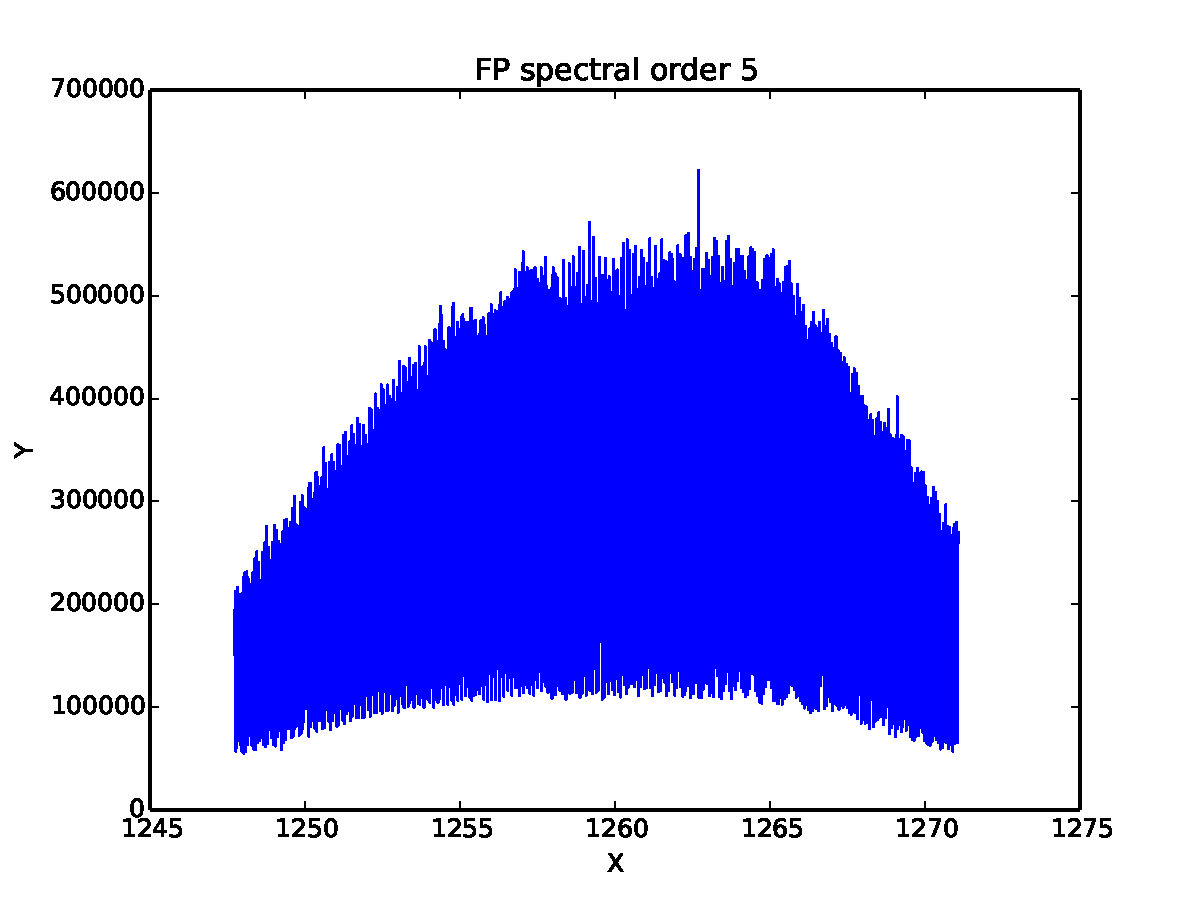
\includegraphics[width=.8\textwidth]{figures/cal_DRIFT_RAW_spirou_1}
\caption{Extract FP spectral order. \label{figure:cal_DRIFT_RAW_spirou_1}}
\end{center}
\end{figure}

\begin{figure}
\begin{center}
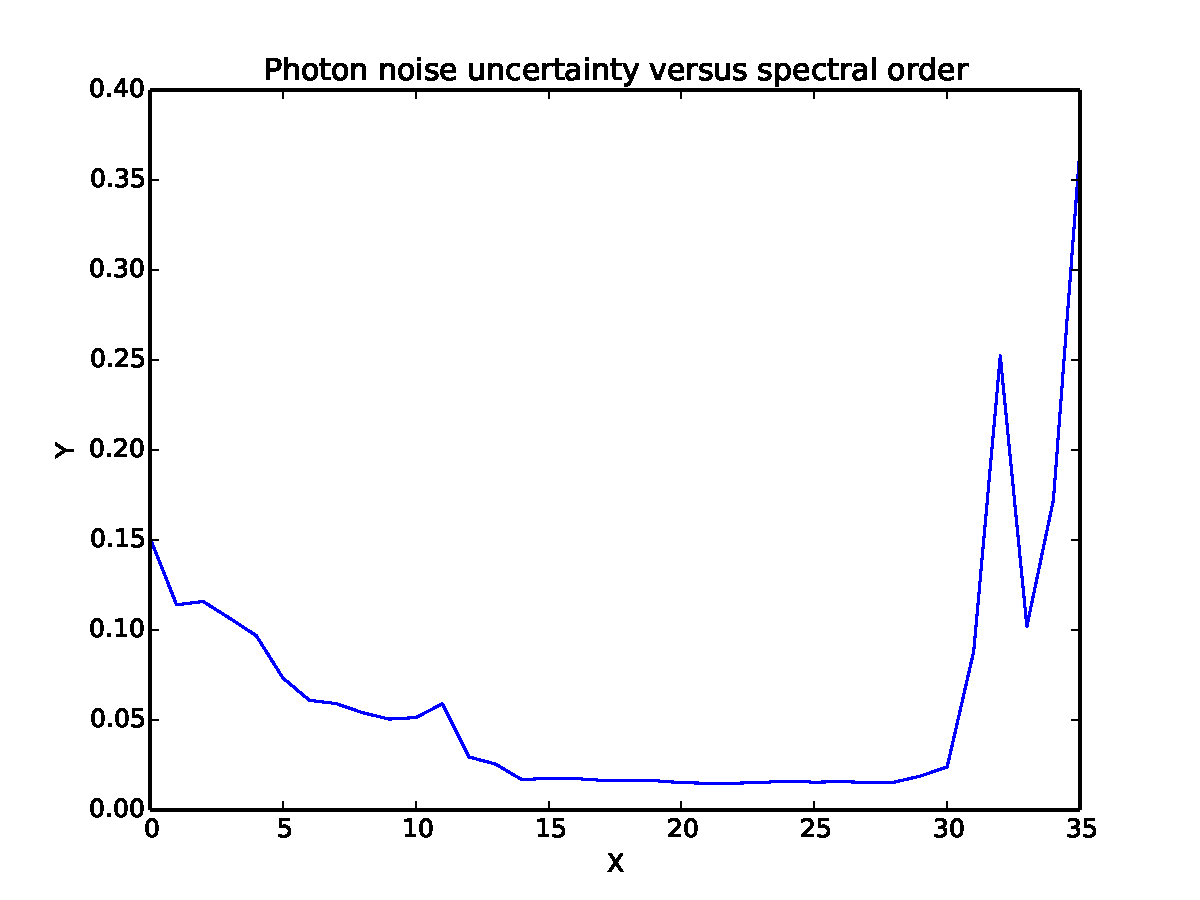
\includegraphics[width=.8\textwidth]{figures/cal_DRIFT_RAW_spirou_2}
\caption{Photon noise uncertain against spectral order. \label{figure:cal_DRIFT_RAW_spirou_2}}
\end{center}
\end{figure}

\begin{figure}
\begin{center}
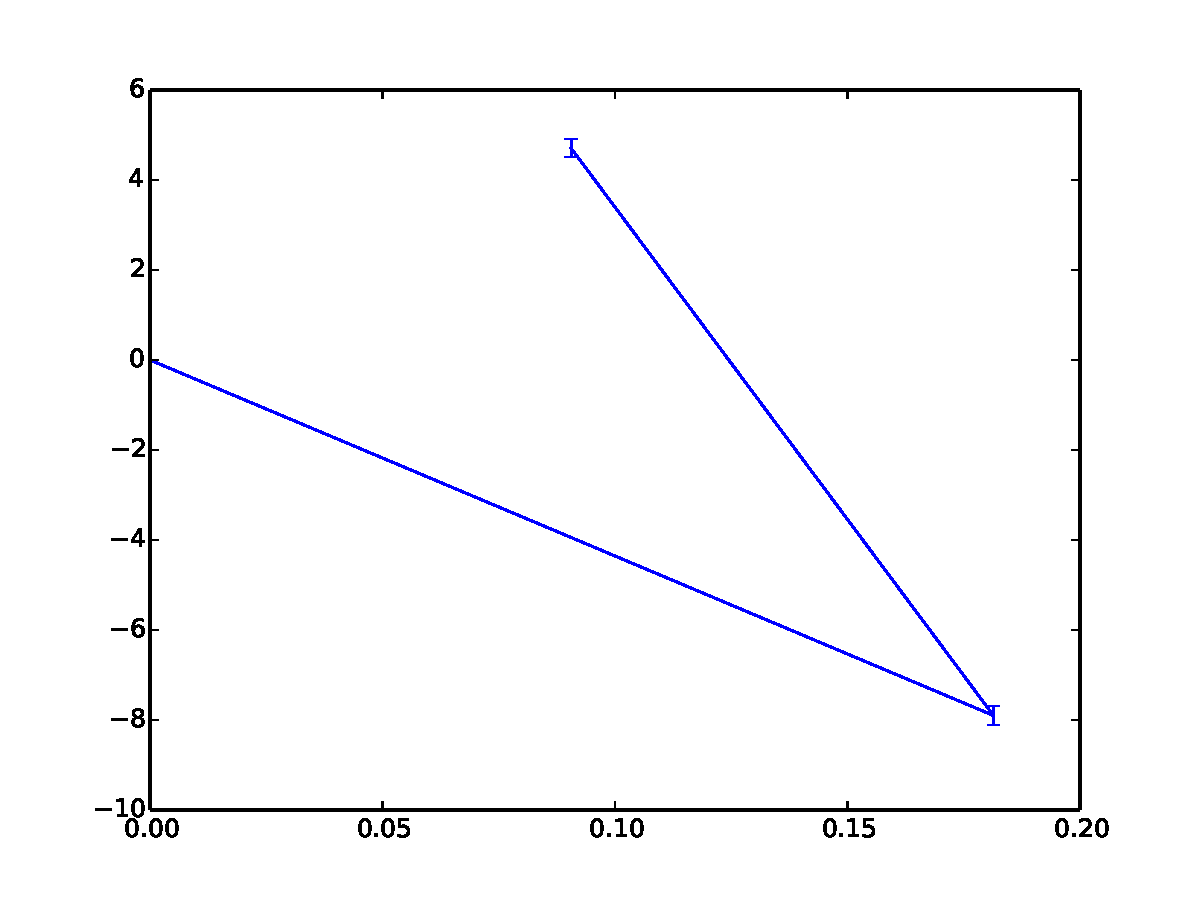
\includegraphics[width=.8\textwidth]{figures/cal_DRIFT_RAW_spirou_3}
\caption{Time interval against median drift. \label{figure:cal_DRIFT_RAW_spirou_3}}
\end{center}
\end{figure}



%----------------------------------------------------------------------------------
\clearpage
\newpage
\section{The cal\_HC\_E2DS\_spirou recipe}
\label{section:cal_HC_E2DS}
% ----------------------------------------------------------------------------------

Wavelength calibration. \\

% % \TODO{Once writen up the new version update this description}

\noindent File prefixes allowed:
\begin{itemize}
	\item hc\_hc*AB.fits
	\item hc\_hc*C.fits
\end{itemize}

\subsection{Summary of procedure}
\begin{enumerate}
	\item Reads lamp line file
	\item Tries to identify lines using guess solution
	\item Cleans list of identified lines
	\item Fits wavelength solution on identified lines
	\item Performs a Littrow test
	\item Writes wavelength solution for fibers
	\item Computes CCF
\end{enumerate}

\subsection{Running cal\_HC\_E2DS\_spirou}

To run cal\_HC\_E2DS\_spirou type:
\begin{lstlisting}[language=bash, style=bashstyle]
cal_HC_E2DS_spirou.py  night_repository  hc_hc*.fits
\end{lstlisting}

\noindent Note: Filenames must start with hc\_hc
\noindent Note: Filenames must include either AB or C

% \subsection{Example working run}

% An example run where everything worked is below:

% \begin{lstlisting}[style=text]
% cal_ .py 20170710 
% \end{lstlisting}

% \subsection{Interactive mode}

% \begin{figure}
% \begin{center}
% \includegraphics[width=.8\textwidth]{figures/}
% \caption{ \label{}}
% \end{center}
% \end{figure}

% ----------------------------------------------------------------------------------
\clearpage
\newpage
\section{The cal\_DRIFT\_E2DS\_spirou recipe}
\label{section:cal_drift_e2ds}
% ----------------------------------------------------------------------------------

Calculates relative (radial velocity) drift between all files and individual files. \\

% \TODO{Once writen up the new version update this description}

\noindent File prefixes allowed:
\begin{itemize}
	\item fp\_fp
\end{itemize}

\subsection{Summary of procedure}
\begin{enumerate}
	\item first file is reference image (must be an E2DS file) extracted using one of the cal\_extract\_RAW recipes
	\item loops around all other `fp\_fp' files in directory
	\item calculates photon noise uncertainty and estimated RV uncertainty on spectrum
	\begin{itemize}
		\item uses wave file
	\end{itemize}
	\item calculates RV drift and mean RV drift between reference (mean of files) and other `fp\_fp' files
	\item saves drift values to file
\end{enumerate}

\subsection{Running cal\_DRIFT\_E2DS\_spirou}

To run cal\_DRIFT\_RAW\_spirou type:
\begin{lstlisting}[language=bash, style=bashstyle]
cal_DRIFT_E2DS_spirou.py  night_repository  filename
\end{lstlisting}

Note: Filenames must start with `fp\_fp' and must be a E2DS file extracted using a cal\_extract\_RAW recipe.

\subsection{Example working run}

An example run where everything worked is below:

\begin{lstlisting}[style=text]
cal_DRIFT_E2DS_spirou.py 20170710 fp_fp02a203_e2ds_AB.fits
||DRS  SPIROU   v   (interactive mode)
19:54:17.9 -   || *****************************************
19:54:17.9 -   || * SPIROU \@(#) Geneva Observatory ()
19:54:17.9 -   || *****************************************
19:54:17.9 -   ||(dir_data_raw)      DRS_DATA_RAW=/scratch/Projects/SPIRou_Pipeline/data/raw/
19:54:17.9 -   ||(dir_data_reduc)    DRS_DATA_REDUC=/scratch/Projects/SPIRou_Pipeline/data/reduced/
19:54:17.9 -   ||(dir_drs_config)    DRS_CONFIG=/scratch/Projects/SPIRou_Pipeline/INTROOT/DRS_SPIROU/config/
19:54:17.9 -   ||(dir_calib_db)      DRS_CALIB_DB=/scratch/Projects/SPIRou_Pipeline/data/calibDB
19:54:17.9 -   ||(dir_data_msg)      DRS_DATA_MSG=/scratch/Projects/SPIRou_Pipeline/data/msg/
19:54:17.9 -   ||(print_log)         DRS_LOG=1         %(0: minimum stdin-out logs)
19:54:17.9 -   ||(plot_graph)        DRS_PLOT=NONE            %(def/undef/trigger)
19:54:17.9 -   ||(used_date)         DRS_USED_DATE=undefined
19:54:17.9 -   ||(working_dir)       DRS_DATA_WORKING=/scratch/Projects/SPIRou_Pipeline/data/tmp/
19:54:17.9 -   ||                    DRS_INTERACTIVE is  set
19:54:17.9 -   |cal_DRIFT_E2DS_spirou:|Now running : cal_DRIFT_E2DS_spirou on file(s):  fp_fp02a203_e2ds_AB.fits
19:54:17.9 -   |cal_DRIFT_E2DS_spirou:|On directory /scratch/Projects/SPIRou_Pipeline/data/raw/20170710
19:54:17.9 -   |cal_DRIFT_E2DS_spirou:|ICDP loaded from: /scratch/Projects/SPIRou_Pipeline/INTROOT/DRS_SPIROU/config/hadmrICDP_SPIROU.py
19:54:17.9 -   |cal_DRIFT_E2DS_spirou:|Reading File: /scratch/Projects/SPIRou_Pipeline/data/reduced/20170710/fp_fp02a203_e2ds_AB.fits
19:54:18.2 -   |cal_DRIFT_E2DS_spirou:|Calibration file: fp_fp02a203_tilt.fits already exists - not copied
19:54:18.2 -   |cal_DRIFT_E2DS_spirou:|Calibration file: dark_flat02f10_loco_C.fits already exists - not copied
19:54:18.9 -   |cal_DRIFT_E2DS_spirou:|Calibration file: dark_flat02f10_order_profil_C.fits already exists - not copied
19:54:19.7 -   |cal_DRIFT_E2DS_spirou:|Calibration file: flat_dark02f10_order_profil_AB.fits already exists - not copied
19:54:19.8 -   |cal_DRIFT_E2DS_spirou:|Calibration file: spirou_wave_ini3.fits already exists - not copied
19:54:20.6 -   |cal_DRIFT_E2DS_spirou:|Calibration file: dark_dark02d406.fits already exists - not copied
19:54:20.7 -   |cal_DRIFT_E2DS_spirou:|Calibration file: dark_flat02f10_flat_C.fits already exists - not copied
19:54:20.7 -   |cal_DRIFT_E2DS_spirou:|Calibration file: flat_dark02f10_flat_AB.fits already exists - not copied
19:54:20.8 -   |cal_DRIFT_E2DS_spirou:|Calibration file: flat_dark02f10_loco_AB.fits already exists - not copied
19:54:21.6 -   |cal_DRIFT_E2DS_spirou:|Calibration file: dark_dark02d406_badpixel.fits already exists - not copied
19:54:21.6 -   |cal_DRIFT_E2DS_spirou:|Reading wavelength solution
19:54:21.6 -   |cal_DRIFT_E2DS_spirou:|Reading Flat-Field
19:54:21.6 -   |cal_DRIFT_E2DS_spirou:|Extraction Reference file  /scratch/Projects/SPIRou_Pipeline/data/reduced/20170710/fp_fp02a203_e2ds_AB.fits
19:54:22.4 - * |cal_DRIFT_E2DS_spirou:|On fiber AB estimated RV uncertainty on spectrum is 0.025 m/s
19:54:22.4 - * |cal_DRIFT_E2DS_spirou:|Nb fp_fp files found on directory =  2
19:54:22.4 -   |cal_DRIFT_E2DS_spirou:|Reading File: /scratch/Projects/SPIRou_Pipeline/data/reduced/20170710/fp_fp03a203_e2ds_AB.fits
19:54:23.0 -   |cal_DRIFT_E2DS_spirou:|Time from ref= 0.09 h  - Drift mean= -2.91 +- 0.036  m/s - Flux ratio= 0.99 - Nb Cosmics= 392
19:54:23.0 -   |cal_DRIFT_E2DS_spirou:|Reading File: /scratch/Projects/SPIRou_Pipeline/data/reduced/20170710/fp_fp04a203_e2ds_AB.fits
19:54:23.6 -   |cal_DRIFT_E2DS_spirou:|Time from ref= 0.18 h  - Drift mean= 10.23 +- 0.036  m/s - Flux ratio= 0.98 - Nb Cosmics= 346
19:54:23.7 -   |cal_DRIFT_E2DS_spirou:|Total drift Peak-To-Peak= 13.135 m/s RMS= 6.567 m/s in 0.18 hour
19:54:23.7 -   |cal_DRIFT_E2DS_spirou:|Drift per orders saved in /scratch/Projects/SPIRou_Pipeline/data/reduced/20170710/fp_fp02a203_e2ds_AB_drift.fits
19:54:24.5 -   |cal_DRIFT_E2DS_spirou:AB|Average Drift saved in /scratch/Projects/SPIRou_Pipeline/data/reduced/20170710/fp_fp02a203_e2ds_AB_drift.tbl Saved
19:54:24.5 - * |cal_DRIFT_E2DS_spirou:|Recipe cal_DRIFT_E2DS_spirou has been  successfully completed

\end{lstlisting}


\subsection{Interactive mode}

\begin{figure}
\begin{center}
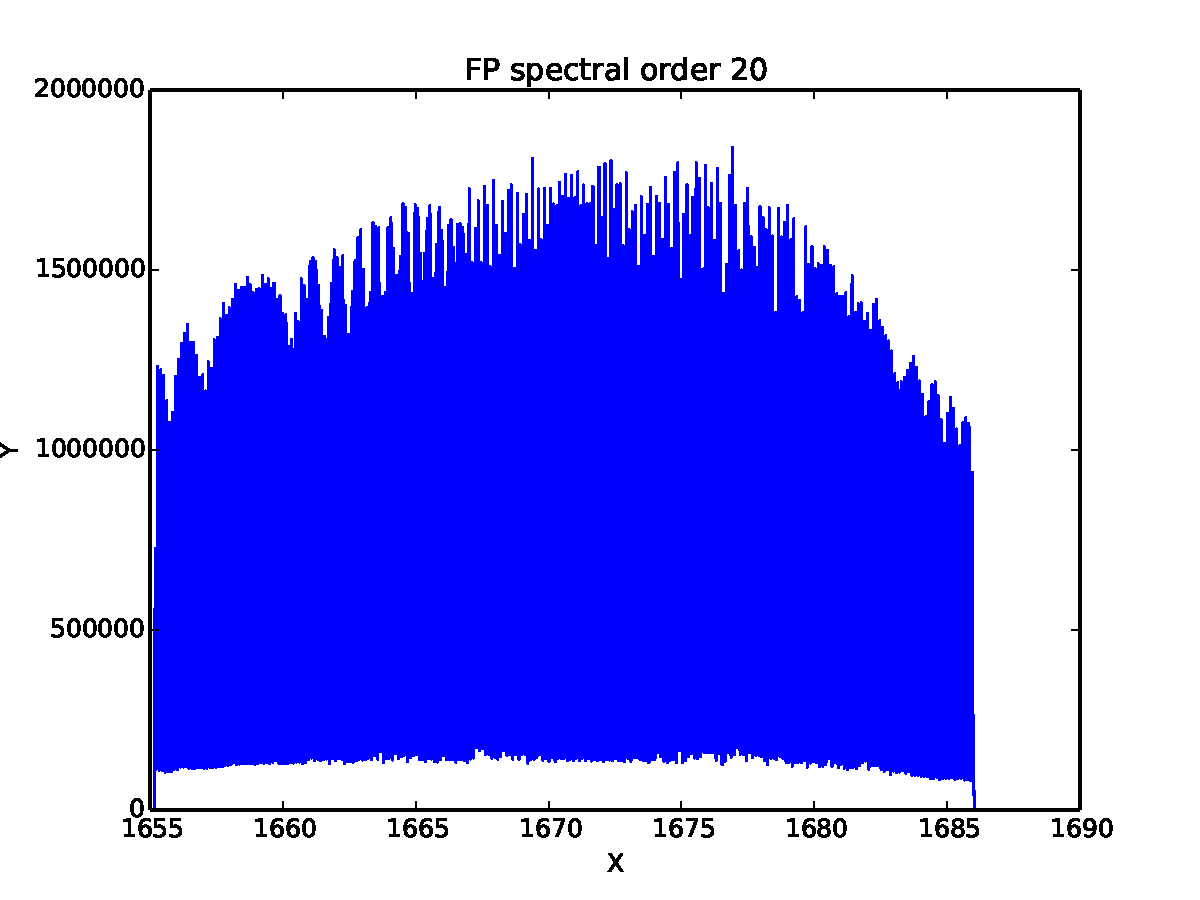
\includegraphics[width=.8\textwidth]{figures/cal_DRIFT_E2DS_spirou_1.pdf}
\caption{The extract FP orders for spectral order 20, x-axis is wavelength and y-axis is extract flux. \label{figure_cal_drift_e2ds_spirou_1}}
\end{center}
\end{figure}

\begin{figure}
\begin{center}
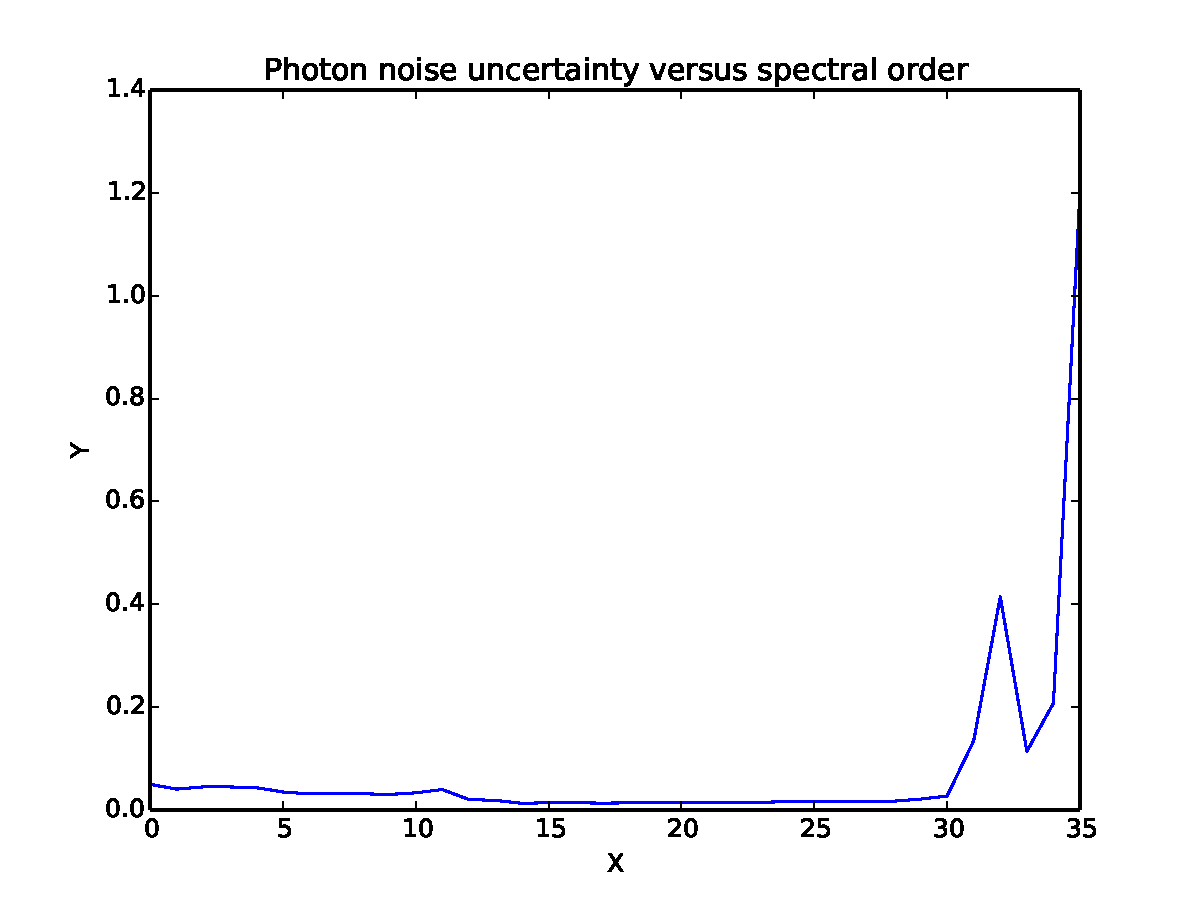
\includegraphics[width=.8\textwidth]{figures/cal_DRIFT_E2DS_spirou_2.pdf}
\caption{Photon noise uncertainty versus spectral order
 \label{figure_cal_drift_e2ds_spirou_2}}
\end{center}
\end{figure}


\begin{figure}
\begin{center}
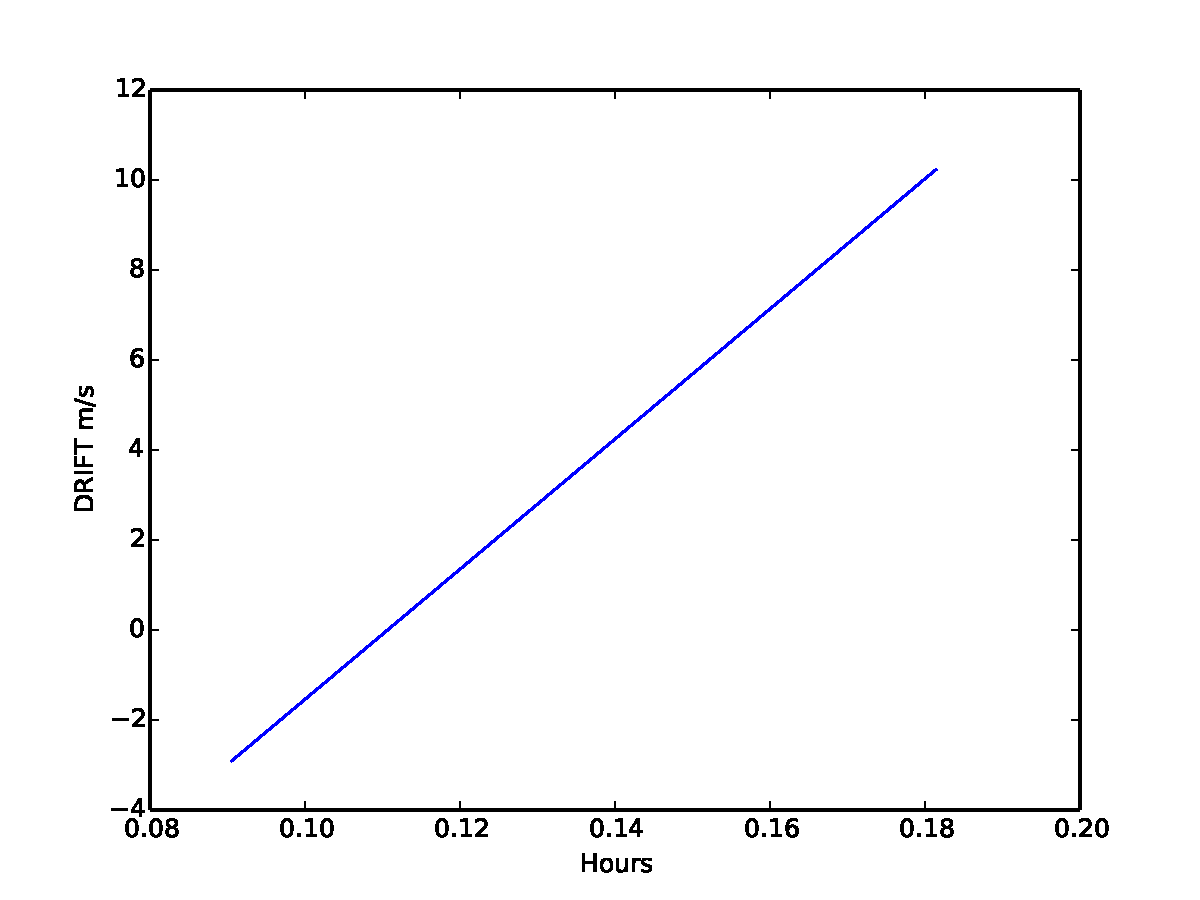
\includegraphics[width=.8\textwidth]{figures/cal_DRIFT_E2DS_spirou_3.pdf}
\caption{Mean drift in m/s against the time from the reference extraction. \label{figure_cal_drift_e2ds_spirou_3}}
\end{center}
\end{figure}

% ----------------------------------------------------------------------------------
\clearpage
\newpage
\section{The cal\_DRIFT-PEAK\_E2DS\_spirou recipe}
\label{section:cal_drift-peak_e2ds}
% ----------------------------------------------------------------------------------

Calculates relative (radial velocity) drift between all files and individual files using a gaussian fitting process to fit the FP peaks. \\

% \TODO{Once writen up the new version update this description}

\noindent File prefixes allowed:
\begin{itemize}
	\item fp\_fp
\end{itemize}

\subsection{Summary of procedure}
\begin{enumerate}
	\item first file is reference image
	\item resizes the image
	\item background correction
	\item Identifies FP peaks in reference file
	\item Creates a reference ascii file that contains the positions of the FP peaks
	\item Removes lines with suspicious widths
	\item loops around all other *\_e2ds\_\definevariable{fiber}.fits files
	\item Gets the centroid of all peaks using Gaussian fitting
	\item Performs a Pearson R test to look for issues with extraction and/or illumination
	\item Performs sigma clipping on measured drift
	\item Saves drifts to file
\end{enumerate}

\subsection{Running cal\_DRIFT-PEAK\_E2DS\_spirou}

To run cal\_DRIFT-PEAK\_E2DS\_spirou type:
\begin{lstlisting}[language=bash, style=bashstyle]
cal_DRIFT-PEAK_E2DS_spirou.py  night_repository fp_fp*.fits
\end{lstlisting}

\noindent Note: Filenames must start with fp\_fp.

\subsection{Example working run}

An example run where everything worked is below:

\begin{lstlisting}[style=text]
cal_DRIFT-PEAK_E2DS_spirou.py 20170710 fp_fp02a203_e2ds_AB.fits
||DRS  SPIROU   v   (interactive mode)
20:15:42.9 -   || *****************************************
20:15:42.9 -   || * SPIROU \@(#) Geneva Observatory ()
20:15:42.9 -   || *****************************************
20:15:42.9 -   ||(dir_data_raw)      DRS_DATA_RAW=/scratch/Projects/SPIRou_Pipeline/data/raw/
20:15:42.9 -   ||(dir_data_reduc)    DRS_DATA_REDUC=/scratch/Projects/SPIRou_Pipeline/data/reduced/
20:15:42.9 -   ||(dir_drs_config)    DRS_CONFIG=/scratch/Projects/SPIRou_Pipeline/INTROOT/DRS_SPIROU/config/
20:15:42.9 -   ||(dir_calib_db)      DRS_CALIB_DB=/scratch/Projects/SPIRou_Pipeline/data/calibDB
20:15:42.9 -   ||(dir_data_msg)      DRS_DATA_MSG=/scratch/Projects/SPIRou_Pipeline/data/msg/
20:15:42.9 -   ||(print_log)         DRS_LOG=1         %(0: minimum stdin-out logs)
20:15:42.9 -   ||(plot_graph)        DRS_PLOT=NONE            %(def/undef/trigger)
20:15:42.9 -   ||(used_date)         DRS_USED_DATE=undefined
20:15:42.9 -   ||(working_dir)       DRS_DATA_WORKING=/scratch/Projects/SPIRou_Pipeline/data/tmp/
20:15:42.9 -   ||                    DRS_INTERACTIVE is  set
20:15:42.9 -   |cal_DRIFT-PEAK_E2DS_spirou:|Now running : cal_DRIFT-PEAK_E2DS_spirou on file(s):  fp_fp02a203_e2ds_AB.fits
20:15:42.9 -   |cal_DRIFT-PEAK_E2DS_spirou:|On directory /scratch/Projects/SPIRou_Pipeline/data/raw/20170710
20:15:43.0 -   |cal_DRIFT-PEAK_E2DS_spirou:|ICDP loaded from: /scratch/Projects/SPIRou_Pipeline/INTROOT/DRS_SPIROU/config/hadmrICDP_SPIROU.py
20:15:43.0 -   |cal_DRIFT-PEAK_E2DS_spirou:|Reading File: /scratch/Projects/SPIRou_Pipeline/data/reduced/20170710/fp_fp02a203_e2ds_AB.fits
20:15:43.1 -   |cal_DRIFT-PEAK_E2DS_spirou:|Calibration file: fp_fp02a203_tilt.fits already exists - not copied
20:15:43.1 -   |cal_DRIFT-PEAK_E2DS_spirou:|Calibration file: dark_flat02f10_loco_C.fits already exists - not copied
20:15:43.1 -   |cal_DRIFT-PEAK_E2DS_spirou:|Calibration file: dark_flat02f10_order_profil_C.fits already exists - not copied
20:15:43.2 -   |cal_DRIFT-PEAK_E2DS_spirou:|Calibration file: flat_dark02f10_order_profil_AB.fits already exists - not copied
20:15:43.2 -   |cal_DRIFT-PEAK_E2DS_spirou:|Calibration file: spirou_wave_ini3.fits already exists - not copied
20:15:43.2 -   |cal_DRIFT-PEAK_E2DS_spirou:|Calibration file: dark_dark02d406.fits already exists - not copied
20:15:43.2 -   |cal_DRIFT-PEAK_E2DS_spirou:|Calibration file: dark_flat02f10_flat_C.fits already exists - not copied
20:15:43.2 -   |cal_DRIFT-PEAK_E2DS_spirou:|Calibration file: flat_dark02f10_flat_AB.fits already exists - not copied
20:15:43.2 -   |cal_DRIFT-PEAK_E2DS_spirou:|Calibration file: flat_dark02f10_loco_AB.fits already exists - not copied
20:15:43.3 -   |cal_DRIFT-PEAK_E2DS_spirou:|Calibration file: dark_dark02d406_badpixel.fits already exists - not copied
20:15:43.3 -   |cal_DRIFT-PEAK_E2DS_spirou:|Reading wavelength solution 
20:15:43.3 -   |cal_DRIFT-PEAK_E2DS_spirou:|Perform background correction 
20:15:43.7 -   |cal_DRIFT-PEAK_E2DS_spirou:|Identification of FP peaks in the Reference file  /scratch/Projects/SPIRou_Pipeline/data/reduced/20170710/fp_fp02a203_e2ds_AB.fits
20:15:44.3 -   |cal_DRIFT-PEAK_E2DS_spirou:|Order 0 : 389 peaks found
20:15:44.7 -   |cal_DRIFT-PEAK_E2DS_spirou:|Order 1 : 383 peaks found
20:15:45.1 -   |cal_DRIFT-PEAK_E2DS_spirou:|Order 2 : 377 peaks found
20:15:45.4 -   |cal_DRIFT-PEAK_E2DS_spirou:|Order 3 : 371 peaks found
20:15:45.7 -   |cal_DRIFT-PEAK_E2DS_spirou:|Order 4 : 366 peaks found
20:15:46.0 -   |cal_DRIFT-PEAK_E2DS_spirou:|Order 5 : 359 peaks found
20:15:46.4 -   |cal_DRIFT-PEAK_E2DS_spirou:|Order 6 : 353 peaks found
20:15:46.8 -   |cal_DRIFT-PEAK_E2DS_spirou:|Order 7 : 348 peaks found
20:15:47.2 -   |cal_DRIFT-PEAK_E2DS_spirou:|Order 8 : 341 peaks found
20:15:47.5 -   |cal_DRIFT-PEAK_E2DS_spirou:|Order 9 : 335 peaks found
20:15:47.7 -   |cal_DRIFT-PEAK_E2DS_spirou:|Order 10 : 327 peaks found
20:15:48.0 -   |cal_DRIFT-PEAK_E2DS_spirou:|Order 11 : 324 peaks found
20:15:48.3 -   |cal_DRIFT-PEAK_E2DS_spirou:|Order 12 : 317 peaks found
20:15:48.6 -   |cal_DRIFT-PEAK_E2DS_spirou:|Order 13 : 311 peaks found
20:15:48.8 -   |cal_DRIFT-PEAK_E2DS_spirou:|Order 14 : 306 peaks found
20:15:49.1 -   |cal_DRIFT-PEAK_E2DS_spirou:|Order 15 : 300 peaks found
20:15:49.4 -   |cal_DRIFT-PEAK_E2DS_spirou:|Order 16 : 294 peaks found
20:15:49.6 -   |cal_DRIFT-PEAK_E2DS_spirou:|Order 17 : 288 peaks found
20:15:49.9 -   |cal_DRIFT-PEAK_E2DS_spirou:|Order 18 : 283 peaks found
20:15:50.1 -   |cal_DRIFT-PEAK_E2DS_spirou:|Order 19 : 277 peaks found
20:15:50.4 -   |cal_DRIFT-PEAK_E2DS_spirou:|Order 20 : 270 peaks found
20:15:50.6 -   |cal_DRIFT-PEAK_E2DS_spirou:|Order 21 : 264 peaks found
20:15:50.9 -   |cal_DRIFT-PEAK_E2DS_spirou:|Order 22 : 258 peaks found
20:15:51.1 -   |cal_DRIFT-PEAK_E2DS_spirou:|Order 23 : 252 peaks found
20:15:51.3 -   |cal_DRIFT-PEAK_E2DS_spirou:|Order 24 : 246 peaks found
20:15:51.5 -   |cal_DRIFT-PEAK_E2DS_spirou:|Order 25 : 241 peaks found
20:15:51.7 -   |cal_DRIFT-PEAK_E2DS_spirou:|Order 26 : 235 peaks found
20:15:51.9 -   |cal_DRIFT-PEAK_E2DS_spirou:|Order 27 : 229 peaks found
20:15:52.1 -   |cal_DRIFT-PEAK_E2DS_spirou:|Order 28 : 223 peaks found
20:15:52.3 -   |cal_DRIFT-PEAK_E2DS_spirou:|Order 29 : 217 peaks found
20:15:52.5 -   |cal_DRIFT-PEAK_E2DS_spirou:|Order 30 : 211 peaks found
20:15:52.6 -   |cal_DRIFT-PEAK_E2DS_spirou:|Order 31 : 120 peaks found
20:15:52.9 -   |cal_DRIFT-PEAK_E2DS_spirou:|Order 32 : 214 peaks found
20:15:53.0 -   |cal_DRIFT-PEAK_E2DS_spirou:|Order 33 : 193 peaks found
20:15:53.2 -   |cal_DRIFT-PEAK_E2DS_spirou:|Order 34 : 187 peaks found
20:15:54.0 -   |cal_DRIFT-PEAK_E2DS_spirou:|Order 35 : 345 peaks found
20:15:54.0 - * |cal_DRIFT-PEAK_E2DS_spirou:|Total Nb of FP lines found = 10354 
20:15:54.0 - * |cal_DRIFT-PEAK_E2DS_spirou:|Nb of lines removed due to suspicious width = 616 
20:16:00.4 - * |cal_DRIFT-PEAK_E2DS_spirou:|Nb fp_fp files found on directory =  2 
20:16:00.4 -   |cal_DRIFT-PEAK_E2DS_spirou:|Reading File: /scratch/Projects/SPIRou_Pipeline/data/reduced/20170710/fp_fp03a203_e2ds_AB.fits
20:16:07.4 - * |cal_DRIFT-PEAK_E2DS_spirou:|Time from ref= 0.09 h  - Drift mean= -2.53 +- 0.21 m/s
20:16:07.4 -   |cal_DRIFT-PEAK_E2DS_spirou:|Reading File: /scratch/Projects/SPIRou_Pipeline/data/reduced/20170710/fp_fp04a203_e2ds_AB.fits
20:16:13.9 - * |cal_DRIFT-PEAK_E2DS_spirou:|Time from ref= 0.18 h  - Drift mean= 9.44 +- 0.23 m/s
20:16:14.0 -   |cal_DRIFT-PEAK_E2DS_spirou:|Total drift Peak-To-Peak= 11.97 m/s RMS= 5.99 m/s in 0.18 hour 
20:16:14.0 -   |cal_DRIFT-PEAK_E2DS_spirou:|Drift per orders saved in /scratch/Projects/SPIRou_Pipeline/data/reduced/20170710/fp_fp02a203_e2ds_AB_driftnew.fits
20:16:14.9 -   |cal_DRIFT-PEAK_E2DS_spirou:AB|Average Drift saved in /scratch/Projects/SPIRou_Pipeline/data/reduced/20170710/fp_fp02a203_e2ds_AB_driftnew.tbl Saved 
20:16:14.9 - * |cal_DRIFT-PEAK_E2DS_spirou:|Recipe cal_DRIFT-PEAK_E2DS_spirou has been  successfully completed

\end{lstlisting}

\subsection{Interactive mode}

\begin{figure}
\begin{center}
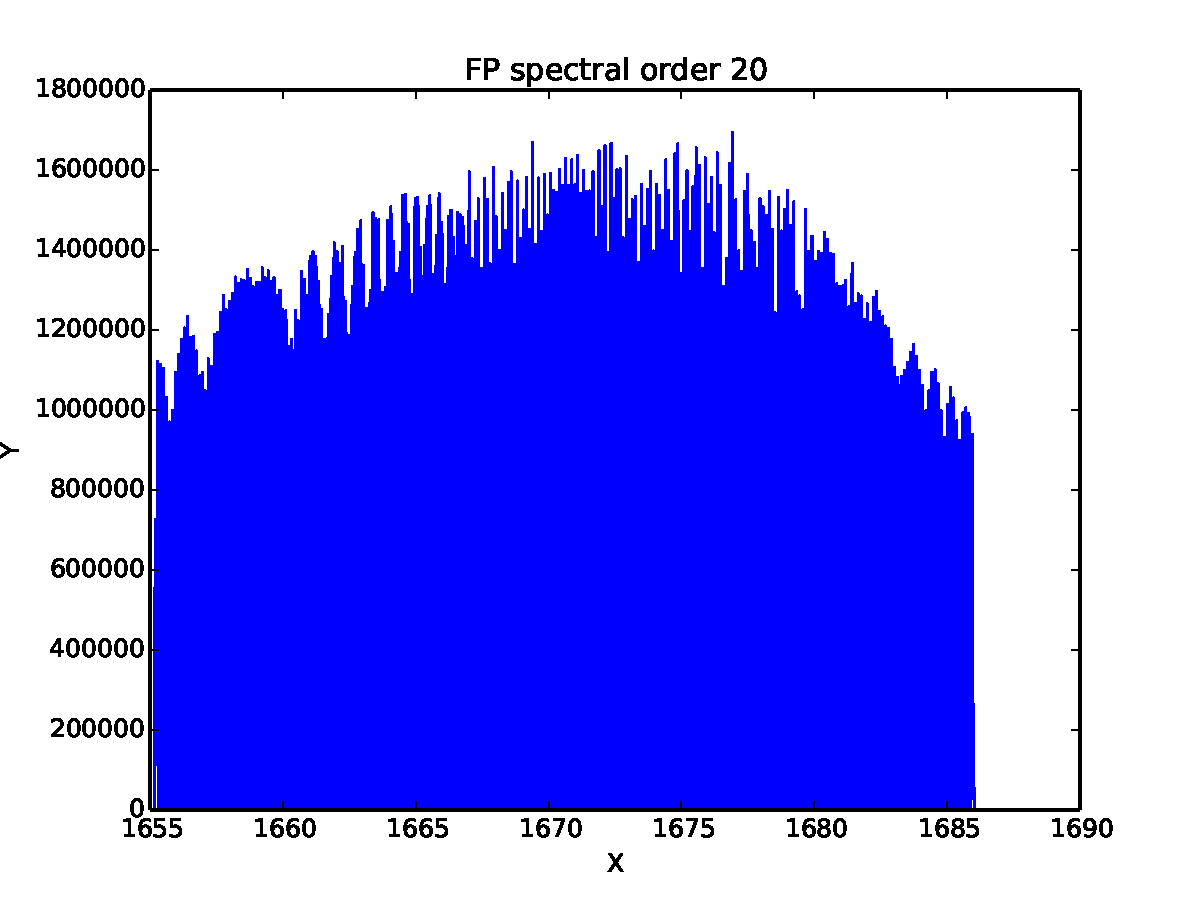
\includegraphics[width=.8\textwidth]{figures/cal_DRIFT-PEAK_E2DS_spirou_1.pdf}
\caption{The extract FP orders for spectral order 20, x-axis is wavelength and y-axis is extract flux. \label{figure:cal_DRIFT-PEAK_E2DS_spirou_1}}
\end{center}
\end{figure}

\begin{figure}
\begin{center}
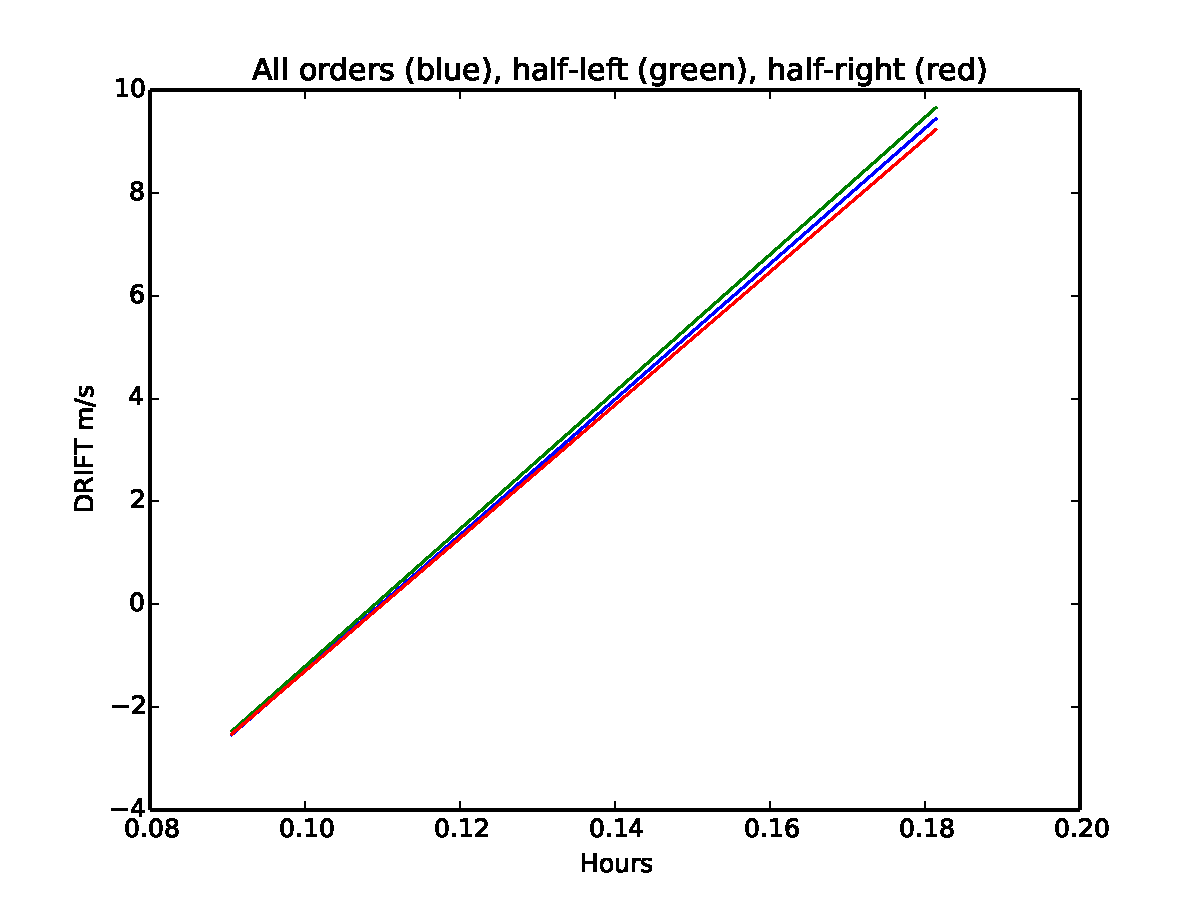
\includegraphics[width=.8\textwidth]{figures/cal_DRIFT-PEAK_E2DS_spirou_2.pdf}
\caption{Mean drift in m/s against the time from the reference extraction for the left side of the orders, the right side of the orders and the whole iamge. \label{figure:cal_DRIFT-PEAK_E2DS_spirou_2}}
\end{center}
\end{figure}
% ----------------------------------------------------------------------------------
\clearpage
\newpage
\section{The cal\_WAVE\_E2DS\_spirou recipe}
\label{section:cal_WAVE_E2DS_spirou}
% ----------------------------------------------------------------------------------

New wavelength solution combining Hollow-Cathode + FP E2DS spectra. \\

% % \TODO{Once writen up the new version update this description}

\noindent File prefixes allowed:
\begin{itemize}
	\item hc\_hc (first file)
	\item fp\_fp (second file)
\end{itemize}

\subsection{Summary of procedure}
\begin{enumerate}
	\item Reads lamp line file
	\item Performs instrumental drift computation
	\item Writes drift to e2ds fits file
	\item Calculates initial wavelength solution
	\item Tries to identify lines using guess solution (x2) 
	\item Cleans list of identified lines (x2)
	\item Fits wavelength solution on identified lines (x2)
	\item Performs a Littrow test (x2)
	\item Writes wavelength solution for fibers
	\item Computes CCF
\end{enumerate}

\subsection{Running cal\_WAVE\_E2DS\_spirou}

To run cal\_WAVE\_E2DS\_spirou type:
\begin{lstlisting}[language=bash, style=bashstyle]
cal_WAVE_E2DS_spirou.py night_repository  hc_hc_*_e2ds_AB.fits    fp_fp_*_e2ds_AB.fits 
\end{lstlisting}

\noindent Note: First file must start with hc\_hc and contain AB or C
\noindent Note: Second file must start with fp\_fp and contain AB or C

% \subsection{Example working run}

% An example run where everything worked is below:

% \begin{lstlisting}[style=text]
% cal_ .py 20170710 
% \end{lstlisting}

% \subsection{Interactive mode}

% \begin{figure}
% \begin{center}
% \includegraphics[width=.8\textwidth]{figures/}
% \caption{ \label{}}
% \end{center}
% \end{figure}


% ----------------------------------------------------------------------------------
\clearpage
\newpage
\section{The cal\_BADPIX\_spirou recipe}
\label{section:cal_BADPIX_spirou}
% ----------------------------------------------------------------------------------

Recipe to generate the bad pixel map. \\

% \TODO{Once writen up the new version update this description}

\noindent File prefixes allowed:
\begin{itemize}
	\item flat\_flat (first file)
	\item dark\_dark (second file)
\end{itemize}

\subsection{Summary of procedure}
\begin{enumerate}
	\item Normalise the flats
	\item Look for isolated hot pixels
	\item Calculate how much pixels deviate compared to expected values
	\item Select hot pixels compared to neighbours
	\item Combine bad pixel map
	\item Save bad pixel mask to file
\end{enumerate}

\subsection{Running cal\_DRIFT\_RAW\_spirou}

To run cal\_DRIFT\_RAW\_spirou type:
\begin{lstlisting}[language=bash, style=bashstyle]
cal_BADPIX_spirou.py night_repository flat_flat*.fits dark_dark*.fits
\end{lstlisting}

\noindent Note: Filenames must start with flat\_flat (first file) and dark\_dark (second file)

\noindent Note: only two files allowed (one flat plus one dark)

\subsection{Example working run}

An example run where everything worked is below:

\begin{lstlisting}[style=text]
cal_BADPIX_spirou.py 20170710 flat_flat02f10.fits dark_dark02d406.fits
||DRS  SPIROU   v   (interactive mode)
15:49:54.7 -   || *****************************************
15:49:54.7 -   || * SPIROU \@(#) Geneva Observatory ()
15:49:54.7 -   || *****************************************
15:49:54.7 -   ||(dir_data_raw)      DRS_DATA_RAW=/scratch/Projects/SPIRou_Pipeline/data/raw/
15:49:54.7 -   ||(dir_data_reduc)    DRS_DATA_REDUC=/scratch/Projects/SPIRou_Pipeline/data/reduced/
15:49:54.7 -   ||(dir_drs_config)    DRS_CONFIG=/scratch/Projects/SPIRou_Pipeline/INTROOT/DRS_SPIROU/config/
15:49:54.7 -   ||(dir_calib_db)      DRS_CALIB_DB=/scratch/Projects/SPIRou_Pipeline/data/calibDB
15:49:54.7 -   ||(dir_data_msg)      DRS_DATA_MSG=/scratch/Projects/SPIRou_Pipeline/data/msg/
15:49:54.7 -   ||(print_log)         DRS_LOG=1         %(0: minimum stdin-out logs)
15:49:54.7 -   ||(plot_graph)        DRS_PLOT=1            %(def/undef/trigger)
15:49:54.7 -   ||(used_date)         DRS_USED_DATE=undefined
15:49:54.7 -   ||(working_dir)       DRS_DATA_WORKING=/scratch/Projects/SPIRou_Pipeline/data/tmp/
15:49:54.7 -   ||                    DRS_INTERACTIVE is  set
15:49:54.7 -   |cal_BADPIX_spirou:+[...]|Now running : cal_BADPIX_spirou on file(s):  flat_flat02f10.fits dark_dark02d406.fits
15:49:54.7 -   |cal_BADPIX_spirou:+[...]|On directory /scratch/Projects/SPIRou_Pipeline/data/raw/20170710
15:49:54.7 -   |cal_BADPIX_spirou:+[...]|ICDP loaded from: /scratch/Projects/SPIRou_Pipeline/INTROOT/DRS_SPIROU/config/hadmrICDP_SPIROU.py
15:49:54.7 - * |cal_BADPIX_spirou:+[...]|Now processing Image TYPE FLAT with cal_BADPIX_spirou recipe
15:49:54.7 - * |cal_BADPIX_spirou:+[...]|Now processing Image TYPE DARK with cal_BADPIX_spirou recipe
15:49:54.7 -   |cal_BADPIX_spirou:+[...]|Reading Flat Image /scratch/Projects/SPIRou_Pipeline/data/raw/20170710/flat_flat02f10.fits
15:49:54.7 -   |cal_BADPIX_spirou:+[...]|Flat Image 2048x2048 loaded
15:49:54.7 -   |cal_BADPIX_spirou:+[...]|Reading Dark Image /scratch/Projects/SPIRou_Pipeline/data/raw/20170710/flat_flat02f10.fits
15:49:54.8 -   |cal_BADPIX_spirou:+[...]|Dark Image 2048x2048 loaded
15:49:54.8 -   |cal_BADPIX_spirou:+[...]|Normalising the flat image
15:49:55.9 -   |cal_BADPIX_spirou:+[...]|Looking for bad pixels
15:49:56.9 -   |cal_BADPIX_spirou:+[...]|Fraction of hot pixels from dark: 3.01 %
15:49:56.9 -   |cal_BADPIX_spirou:+[...]|Fraction of bad pixels from flat: 1.32 %
15:49:56.9 -   |cal_BADPIX_spirou:+[...]|Fraction of NaN pixels in dark: 20.76 %
15:49:56.9 -   |cal_BADPIX_spirou:+[...]|Fraction of NaN pixels in flat: 14.66 %
15:49:56.9 -   |cal_BADPIX_spirou:+[...]|Fraction of bad pixels with all criteria: 24.66 %
15:49:56.9 - * |cal_BADPIX_spirou:+[...]|QUALITY CONTROL SUCCESSFUL - Well Done -
15:49:56.9 -   |cal_BADPIX_spirou:+[...]|Saving Bad Pixel Mask in flat_flat02f10_badpixel.fits
15:49:57.5 - * |cal_BADPIX_spirou:+[...]|Updating Calib Data Base with BADPIX
15:49:57.5 - * |cal_BADPIX_spirou:+[...]|Recipe cal_BADPIX_spirou has been succesfully completed
\end{lstlisting}


% ----------------------------------------------------------------------------------
\clearpage
\newpage
\section{The cal\_CCF\_E2DS\_spirou recipe}
\label{section:cal_CCF_E2DS_spirou}
% ----------------------------------------------------------------------------------

Cross correlation function computation on a E2DS spectra. \\

% \TODO{Once writen up the new version update this description}

\noindent File suffixes allowed:
\begin{itemize}
	\item *e2ds\_AB.fits
\end{itemize}

\subsection{Summary of procedure}
\begin{enumerate}
	\item 
\end{enumerate}

\subsection{Running cal\_DRIFT\_RAW\_spirou}

To run cal\_DRIFT\_RAW\_spirou type:
\begin{lstlisting}[language=bash, style=bashstyle]
cal_CCF_E2DS_spirou.py  night_repository  *e2ds_AB.fits  mask.mas  RV  RANGE  STEP 
\end{lstlisting}

\noindent Note: First argument is a file with suffix *e2ds\_AB.fits
\noindent Note: The mask (Ex : UrNe.mas) is presently loaded locally (in the working directory) 
\noindent Note: RV, RANGE, STEP are the central velocity, half range in velocity and step in km/s of the CCF 

% \subsection{Example working run}

% An example run where everything worked is below:

% \begin{lstlisting}[style=text]
% cal_ .py 20170710 
% \end{lstlisting}

% \subsection{Interactive mode}

% \begin{figure}
% \begin{center}
% \includegraphics[width=.8\textwidth]{figures/}
% \caption{ \label{}}
% \end{center}
% \end{figure}


% % ----------------------------------------------------------------------------------
% \clearpage
% \newpage
% \section{The cal\_ recipe}
% \label{section:cal_}
% % ----------------------------------------------------------------------------------



% % \TODO{Once writen up the new version update this description}

% \noindent File prefixes allowed:
% \begin{itemize}
% 	\item 
% \end{itemize}

% \subsection{Summary of procedure}
% \begin{enumerate}
% 	\item 
% \end{enumerate}

% \subsection{Running cal\_DRIFT\_RAW\_spirou}

% To run cal\_DRIFT\_RAW\_spirou type:
% \begin{lstlisting}[language=bash, style=bashstyle]
% cal_ .py  night_repository  filenames
% \end{lstlisting}

% Note: Filenames must start with 

% \subsection{Example working run}

% An example run where everything worked is below:

% \begin{lstlisting}[style=text]
% cal_ .py 20170710 
% \end{lstlisting}

% \subsection{Interactive mode}

% \begin{figure}
% \begin{center}
% \includegraphics[width=.8\textwidth]{figures/}
% \caption{ \label{}}
% \end{center}
% \end{figure}

% ----------------------------------------------------------------------------------
\clearpage
\newpage
\section{The pol\_spirou recipe}
\label{section:pol_spirou}
% ----------------------------------------------------------------------------------



% ---------------------------------------------------------------
\clearpage
\newpage
\section{Currently unused}
% ---------------------------------------------------------------

\subsection{cal\_loc\_ONE\_spirou}

White lamp exposures on fiber science only (A and B), on fiber C only, or on all of them (ABC). These exposures are used for order localisation and order profil (the pipeline will also need a Fabry-Perot exposure for this last point).

\subsubsection{Running cal\_loc\_ONE\_spirou}

To run cal\_loc\_ONE\_spirou type:
\begin{lstlisting}[language=bash, style=bashstyle]
cal_loc_ONE_spirou.py  night_repository  filename
\end{lstlisting}


\subsection{cal\_FF\_spirou}

A sequence of N white lamp exposures where the two fibres are simultaneously illuminated. This sequence is used by the data reduction pipeline for producing a spectral "master flat-field", monitor the ageing of detector (IR detector loose pixels during its life), monitor the fiber transmission, produce localisation and order profil (the pipeline will also need of exposure « Fabry-Perot » for this last point).

\subsubsection{Running cal\_FF\_spirou}

To run cal\_FF\_spirou type:
\begin{lstlisting}[language=bash, style=bashstyle]
cal_FF_spirou.py  night_repository  filename1 filename2 … filenameN
\end{lstlisting}


\subsection{cal\_WAVE\_spirou}

Hollow Cathode lamp exposures in which the three fibres are simultaneously fed by light from the Hollow Cathode lamps. DRS use each exposure to build a wavelength solution. The instrumental drift with respect to the previous calibration frames is measured.

\subsubsection{Running cal\_WAVE\_spirou}

To run cal\_WAVE\_spiroutype:
\begin{lstlisting}[language=bash, style=bashstyle]
cal_WAVE_spirou.py  night_repository  filename
\end{lstlisting}



\subsection{cal\_FP\_spirou}

Fabry-Perot exposures in which the three fibres are simultaneously fed by light from the Fabry-Perot filter. Each exposure is used to build a wavelength solution and the slit orientation. The instrumental drift with respect to the previous calibration frames is measured. A « super » wavelength solution will be builded in using Hollow Cathode and Fabry-Perot exposures; Hollow Cathode exposures give an absolute reference and Fabry-Perot exposures provide a signal very regularly spaced  in wavelength.

\subsubsection{Running cal\_FP\_spirou}

To run cal\_FP\_spirou type:
\begin{lstlisting}[language=bash, style=bashstyle]
cal_FP_spirou.py  night_repository  filename
\end{lstlisting}
